	\begin{figure}
			\centering
			\subfloat[SHREK]{
				\scalebox{.4}{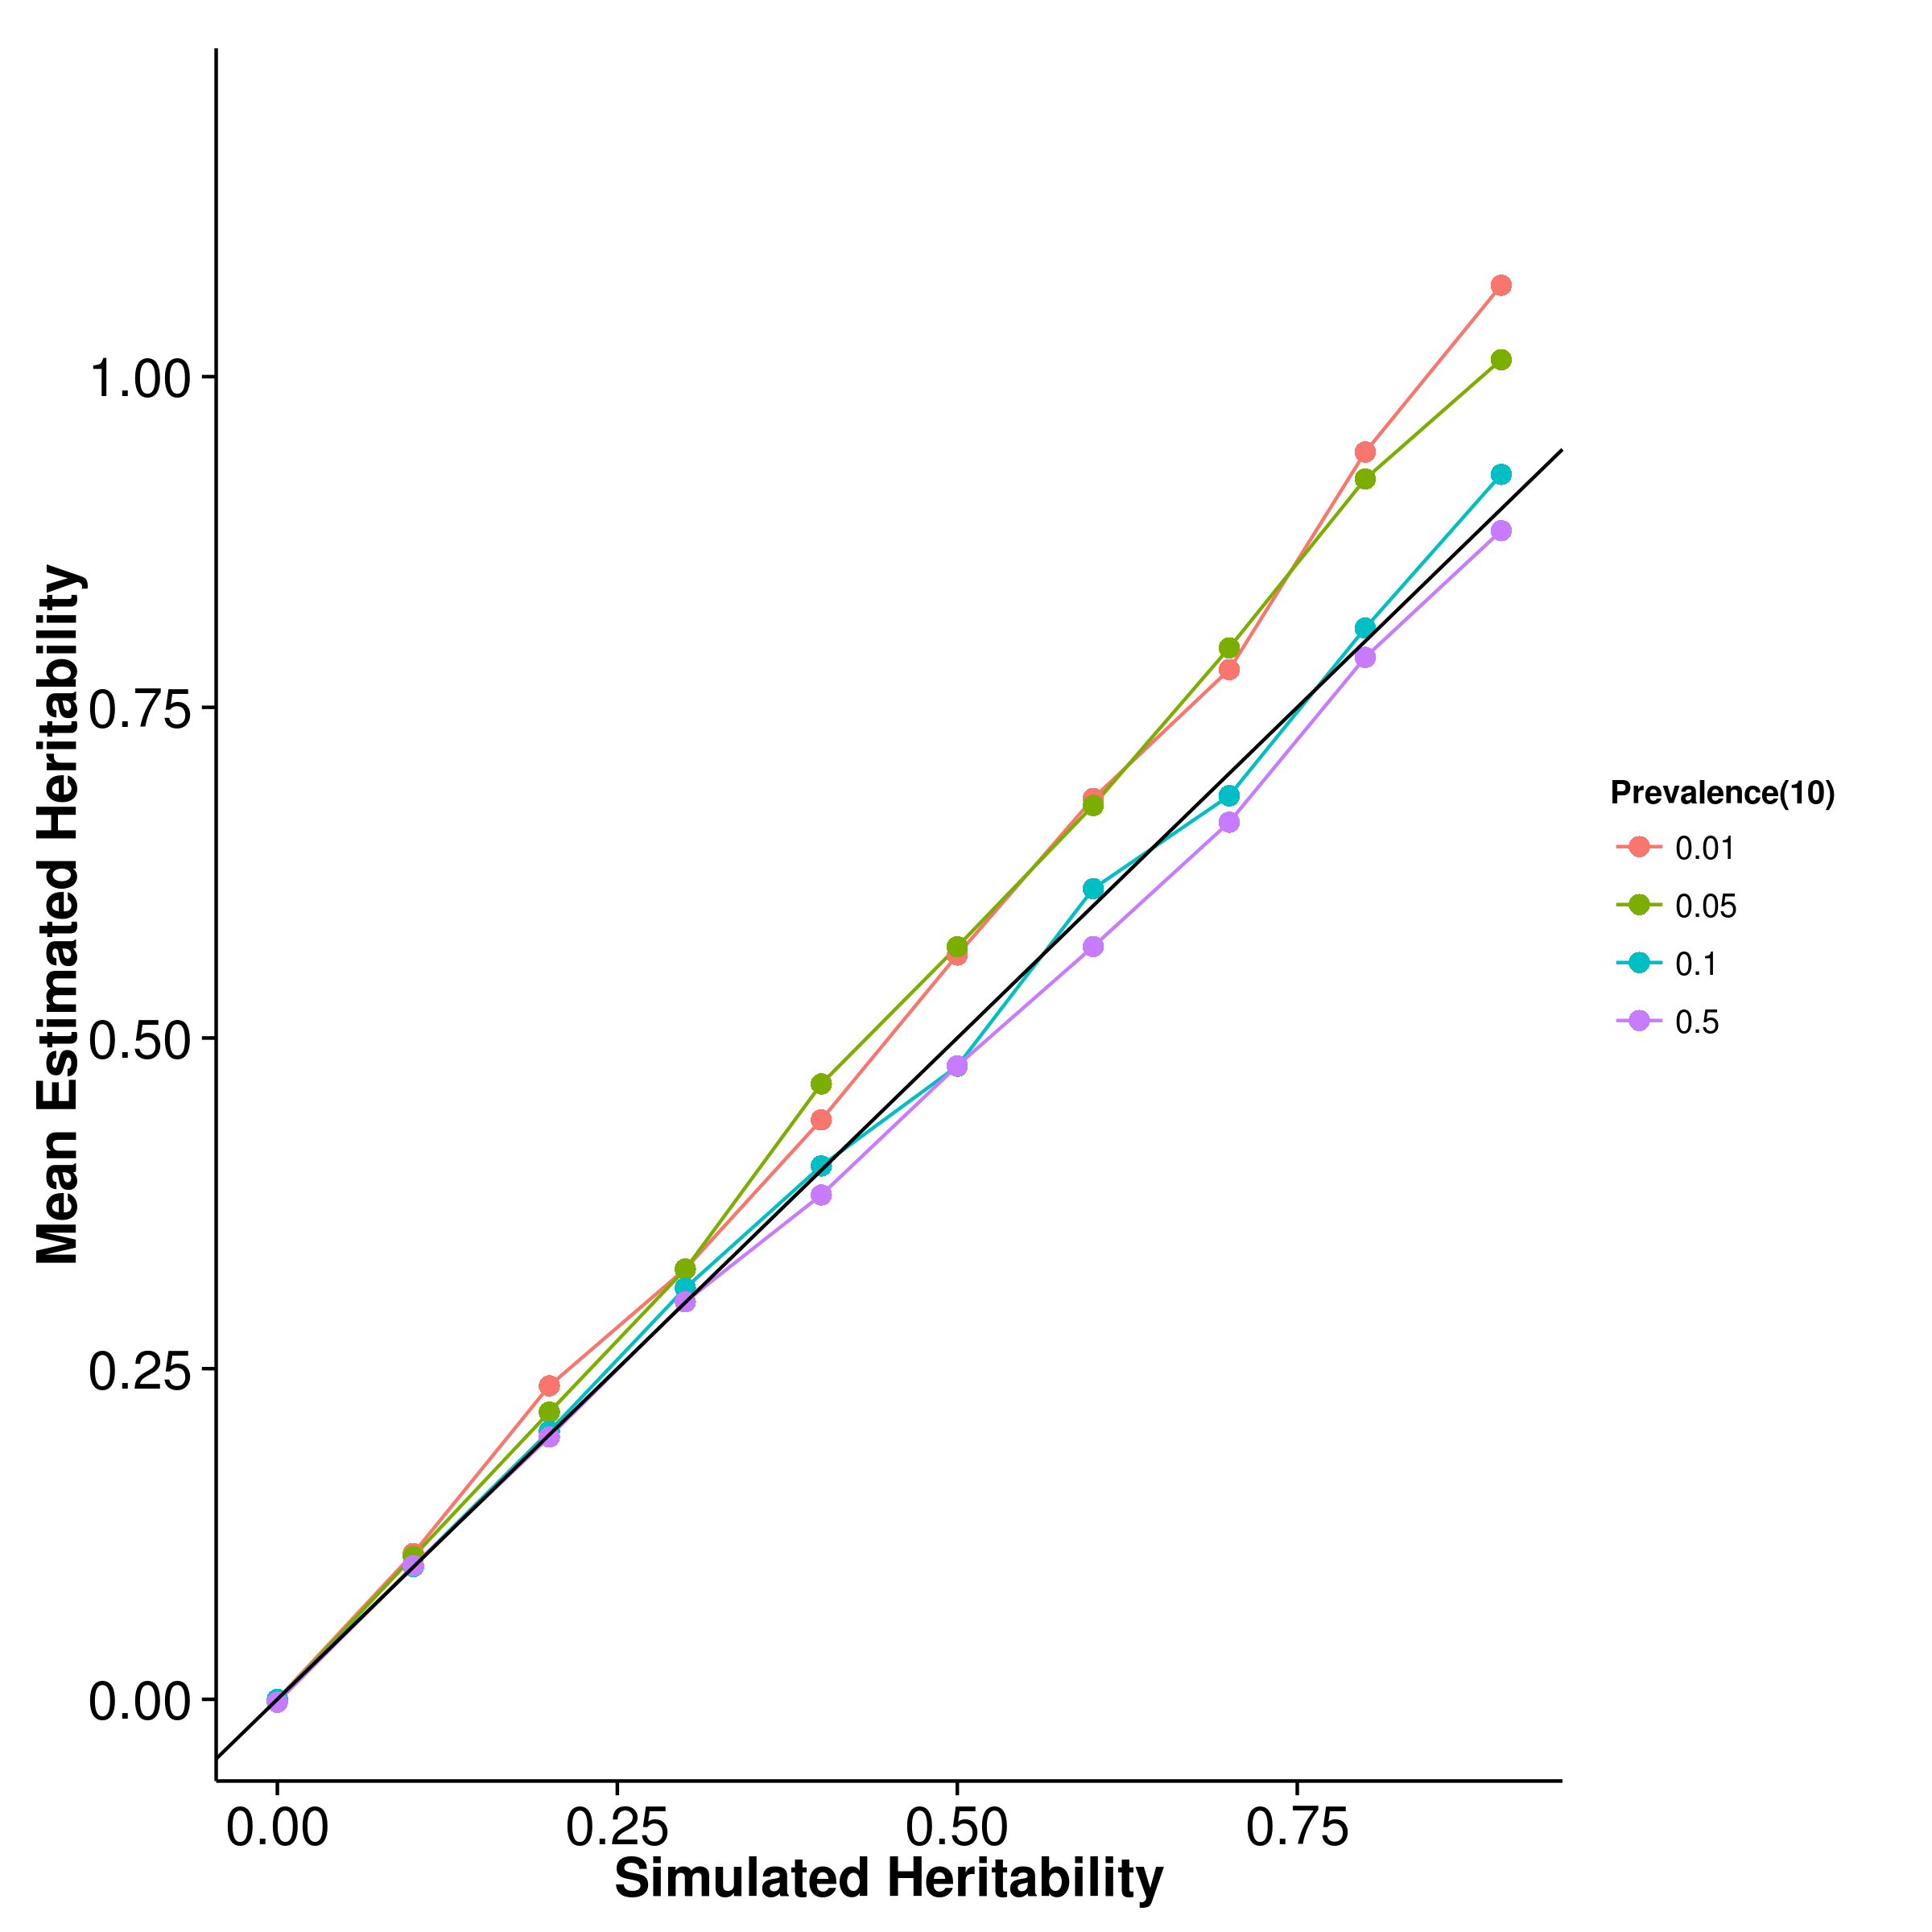
\includegraphics{figure/he_summary/cc_10c/shrek_CC_Rand_mean.png}}
				\label{fig:shrekCC10RandMean}
			}
			\subfloat[GCTA]{
				\scalebox{.4}{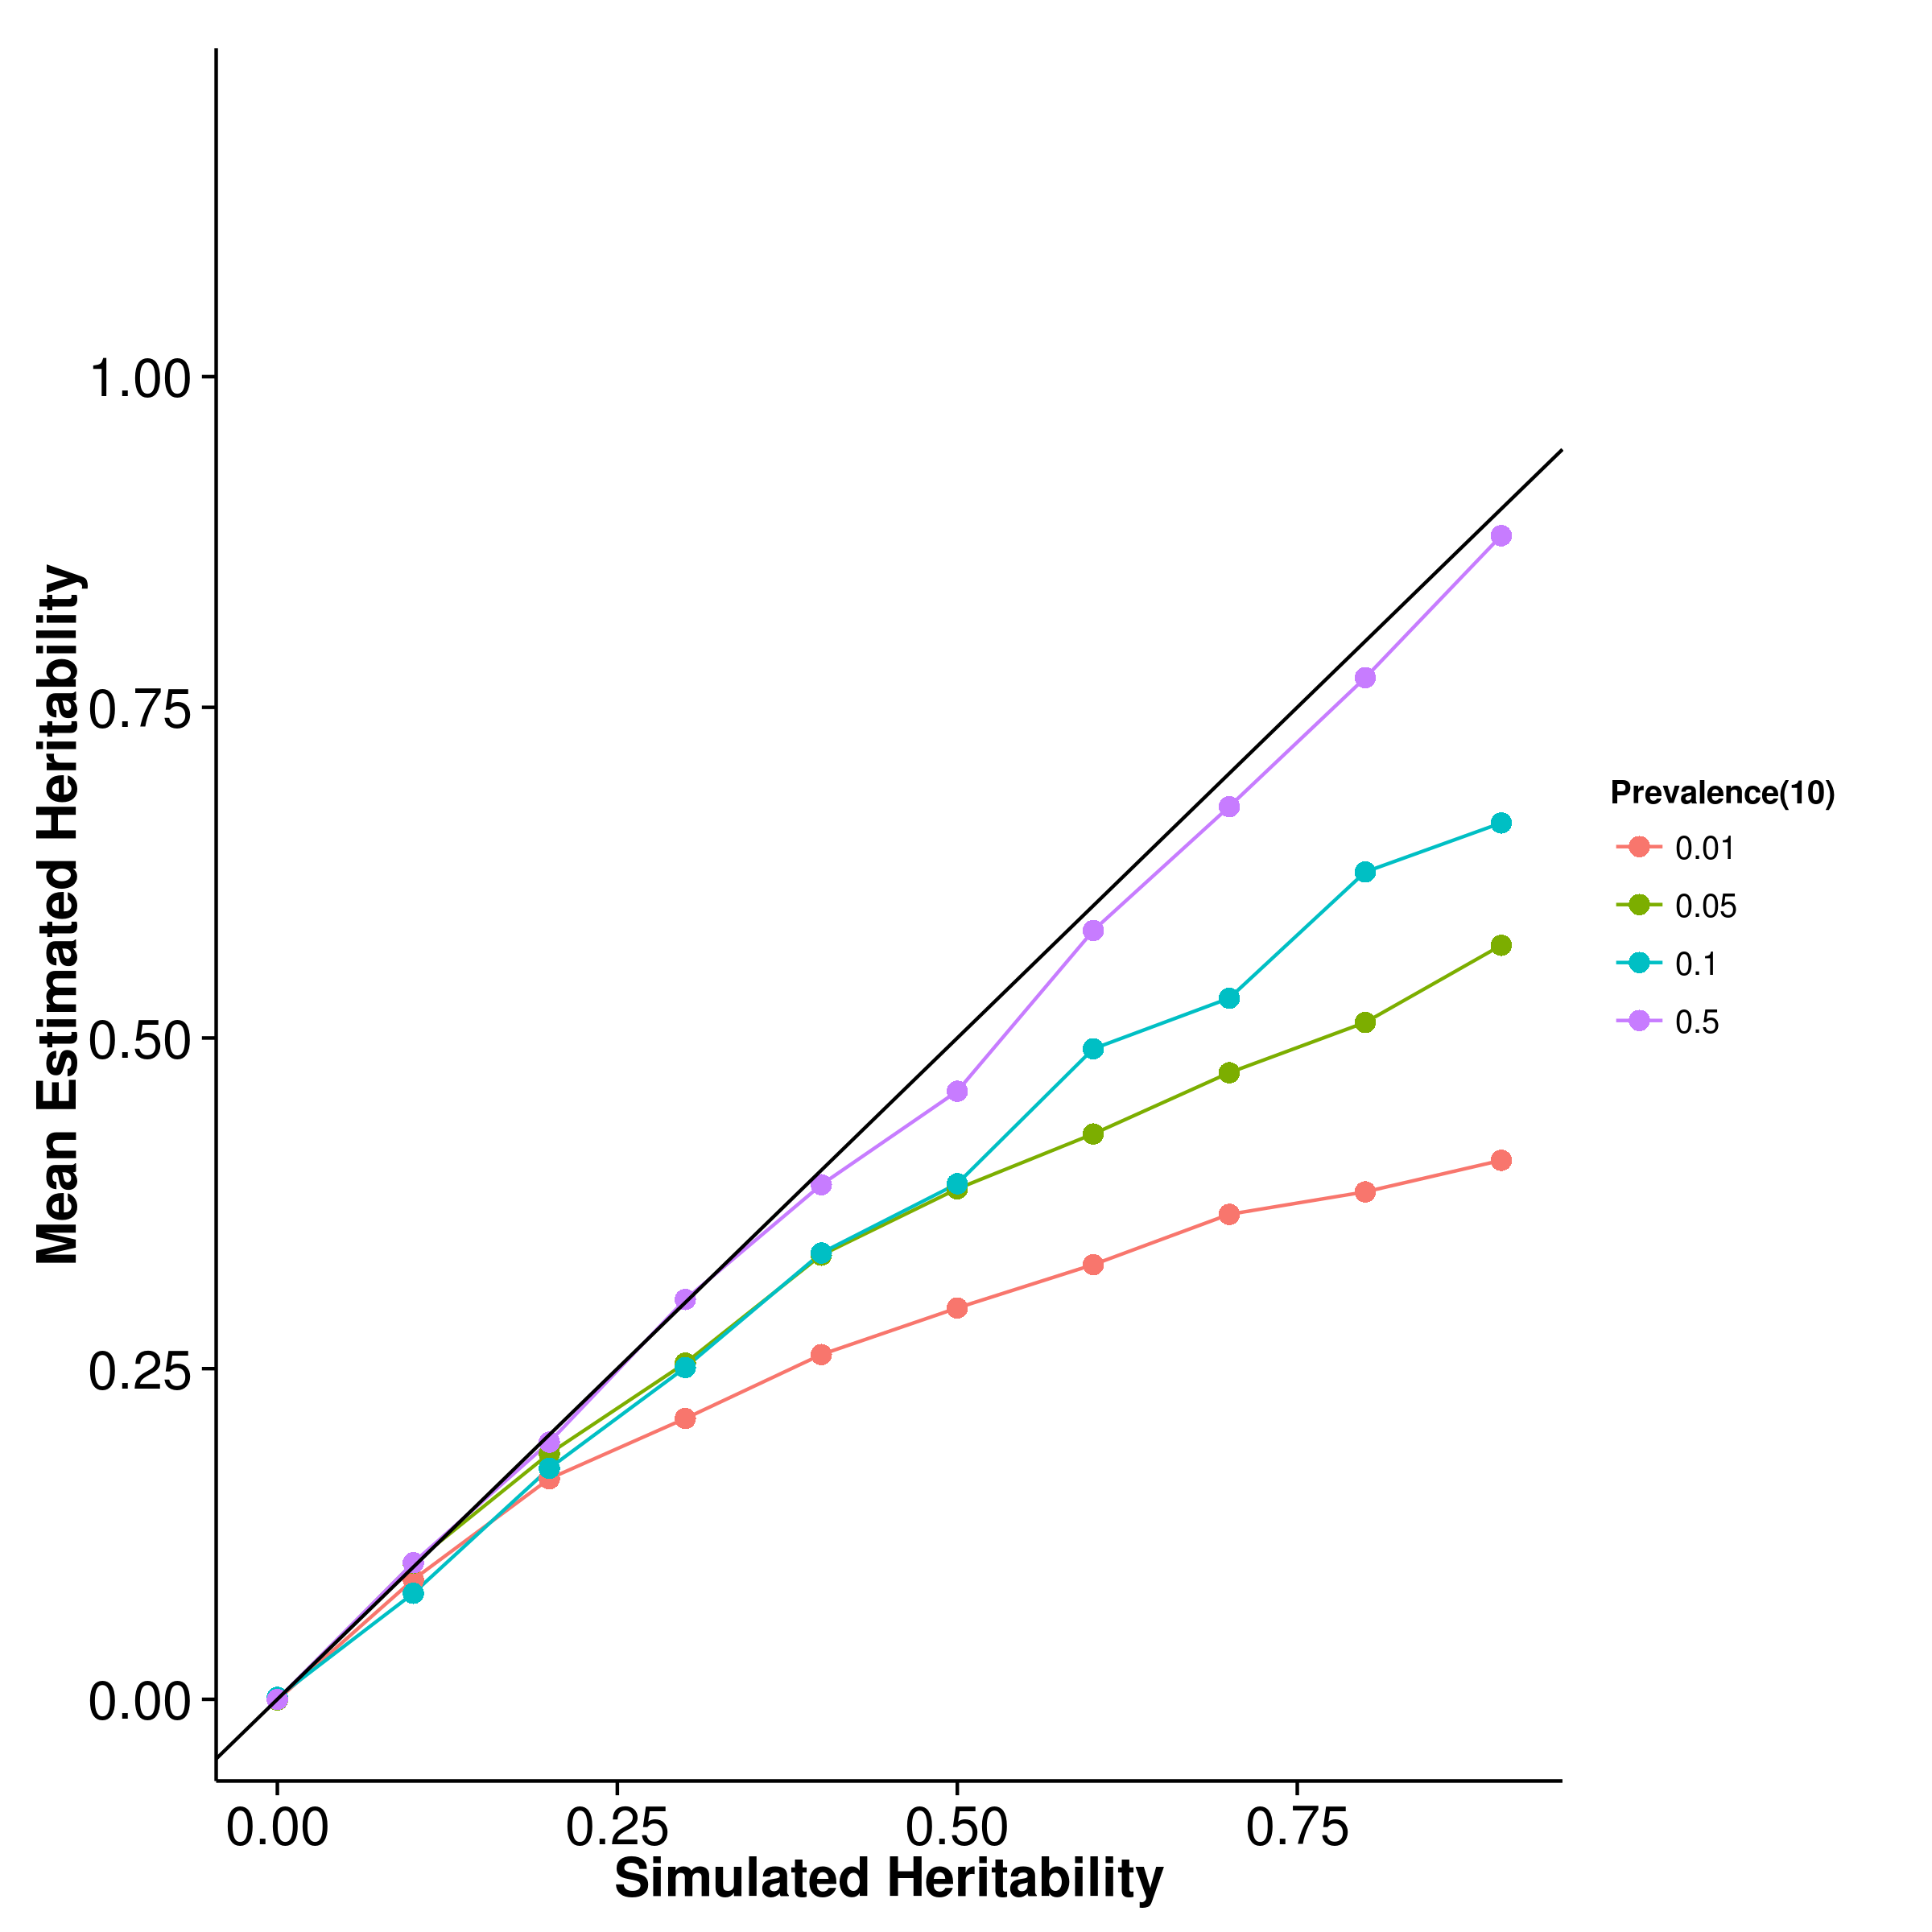
\includegraphics{figure/he_summary/cc_10c/gcta_CC_Rand_mean.png}}
				\label{fig:gctaCC10RandMean}
			}\\
			\subfloat[LDSC with fix intercept]{
				\scalebox{.4}{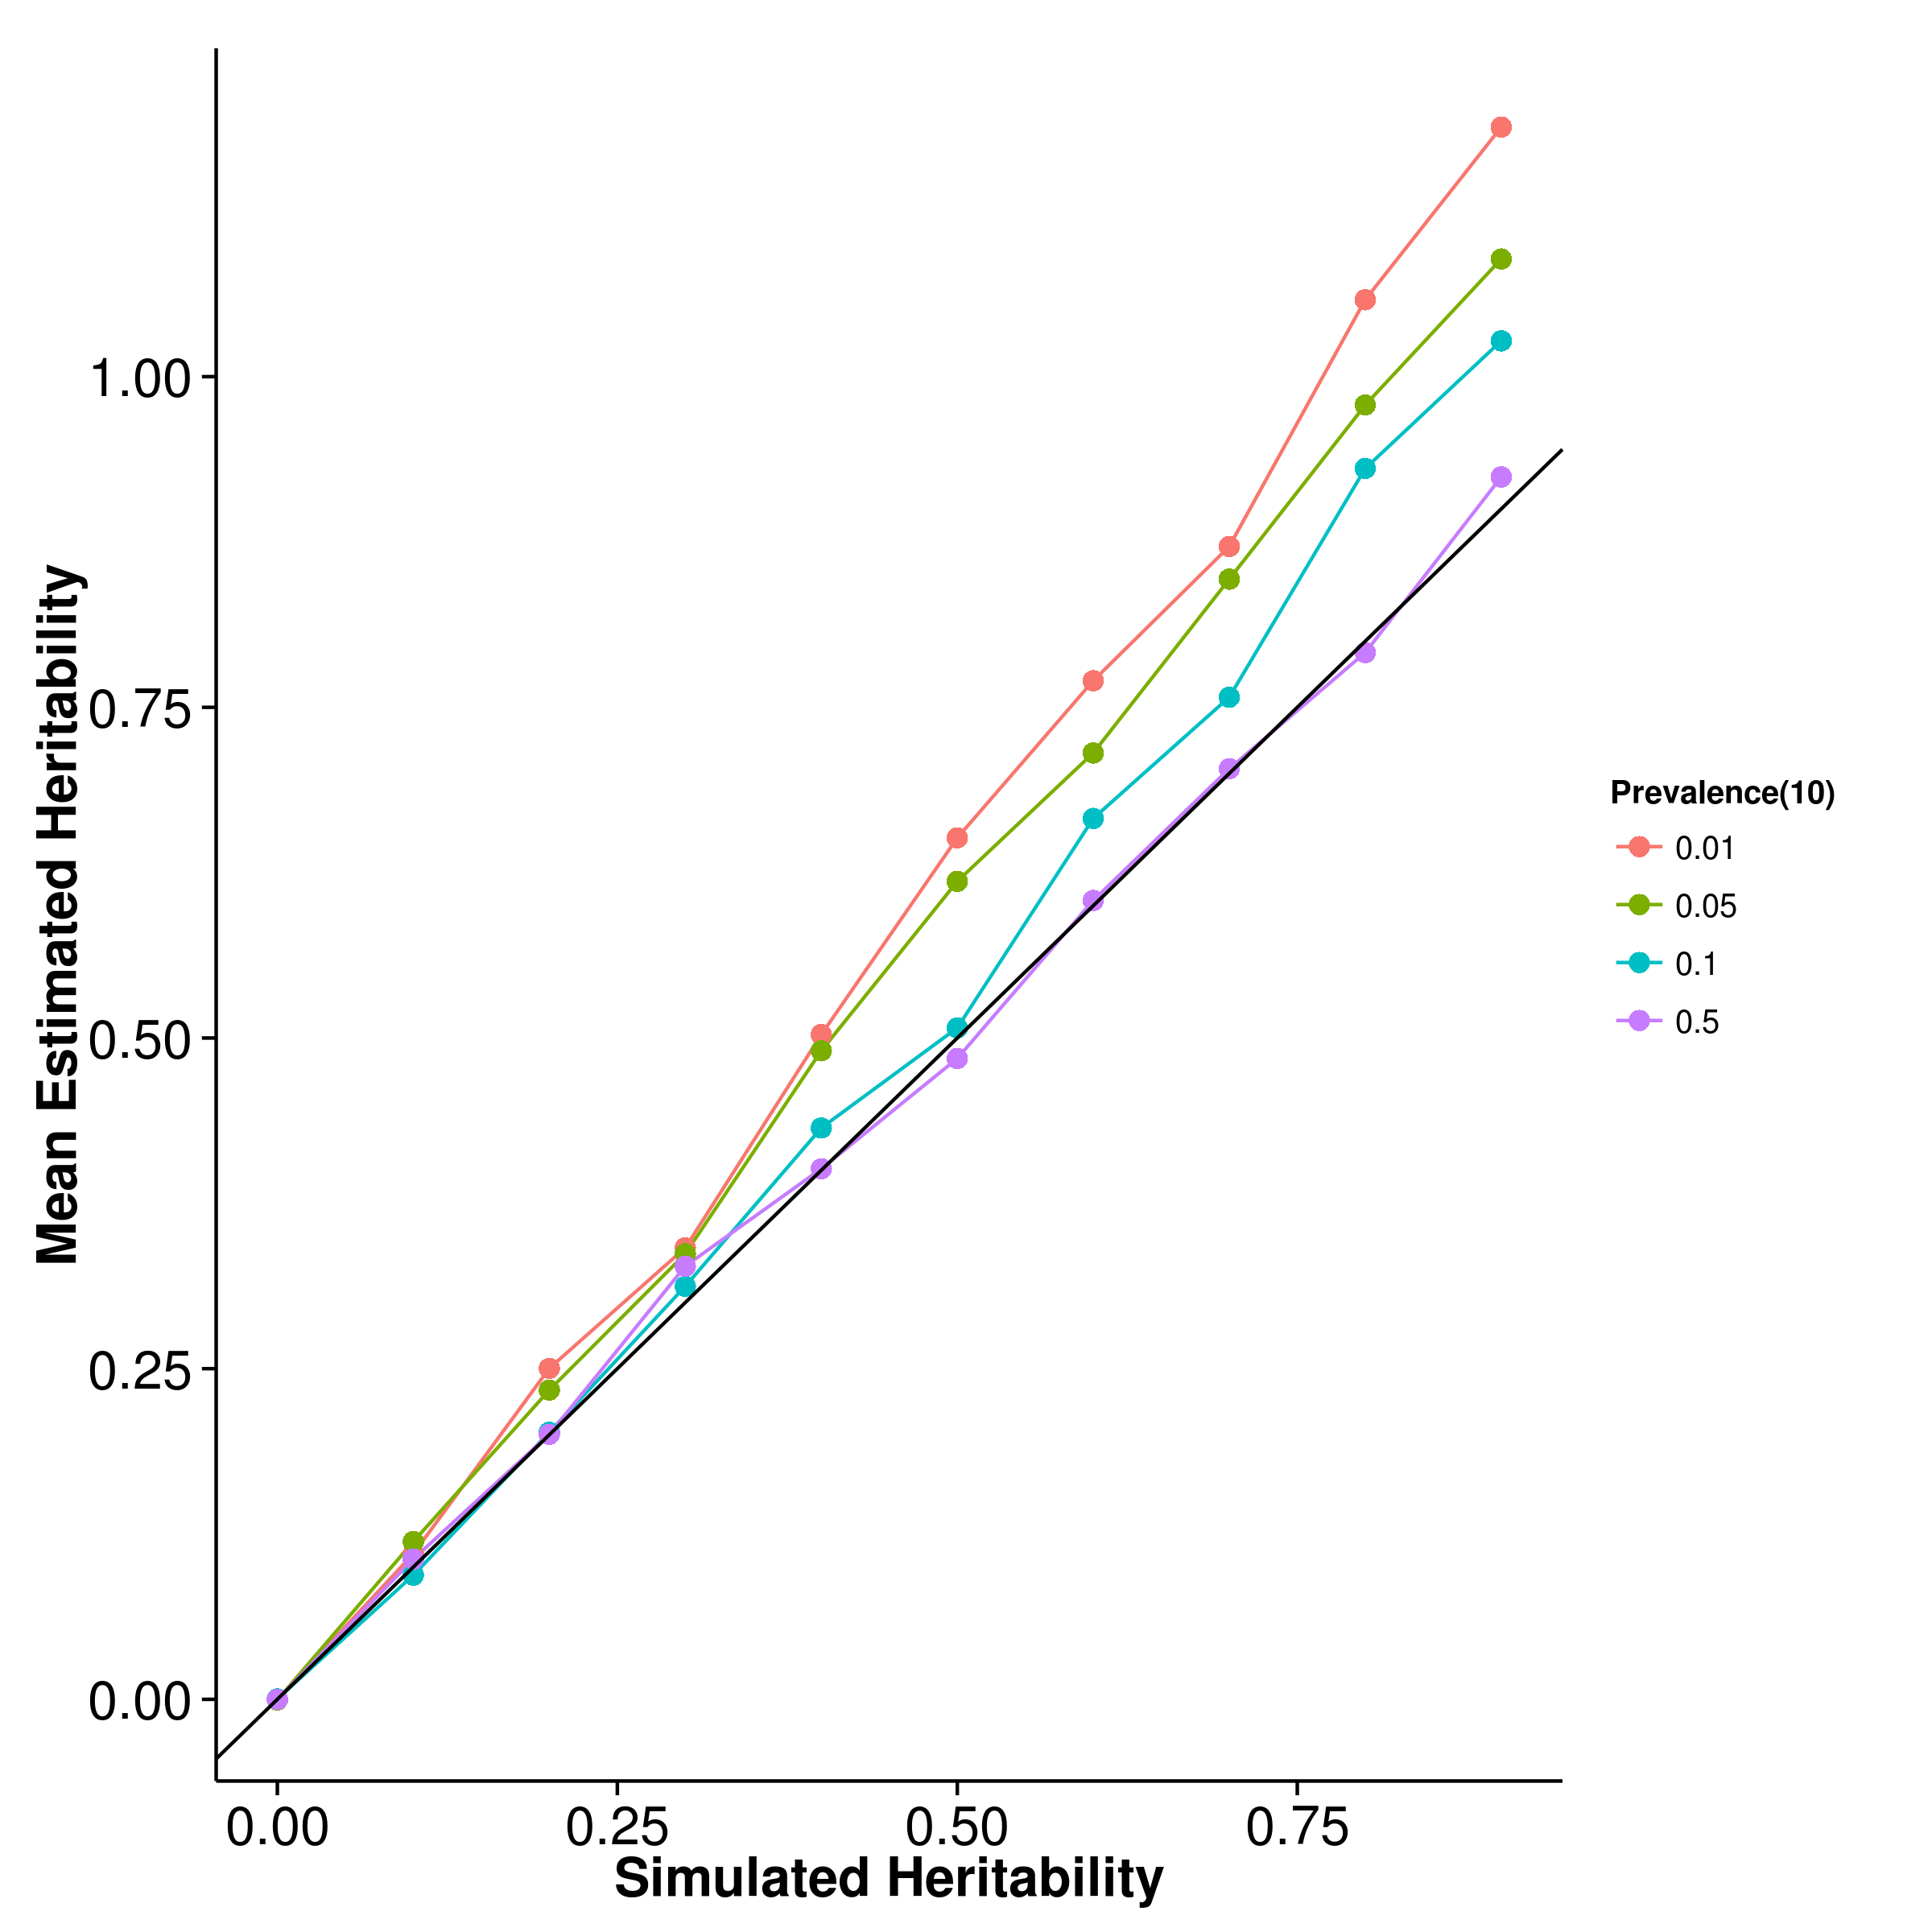
\includegraphics{figure/he_summary/cc_10c/ldsc_CC_Rand_mean.png}}
				\label{fig:ldscCC10RandMean}
			}
			\subfloat[LDSC with intercept estimation]{
				
				\scalebox{.4}{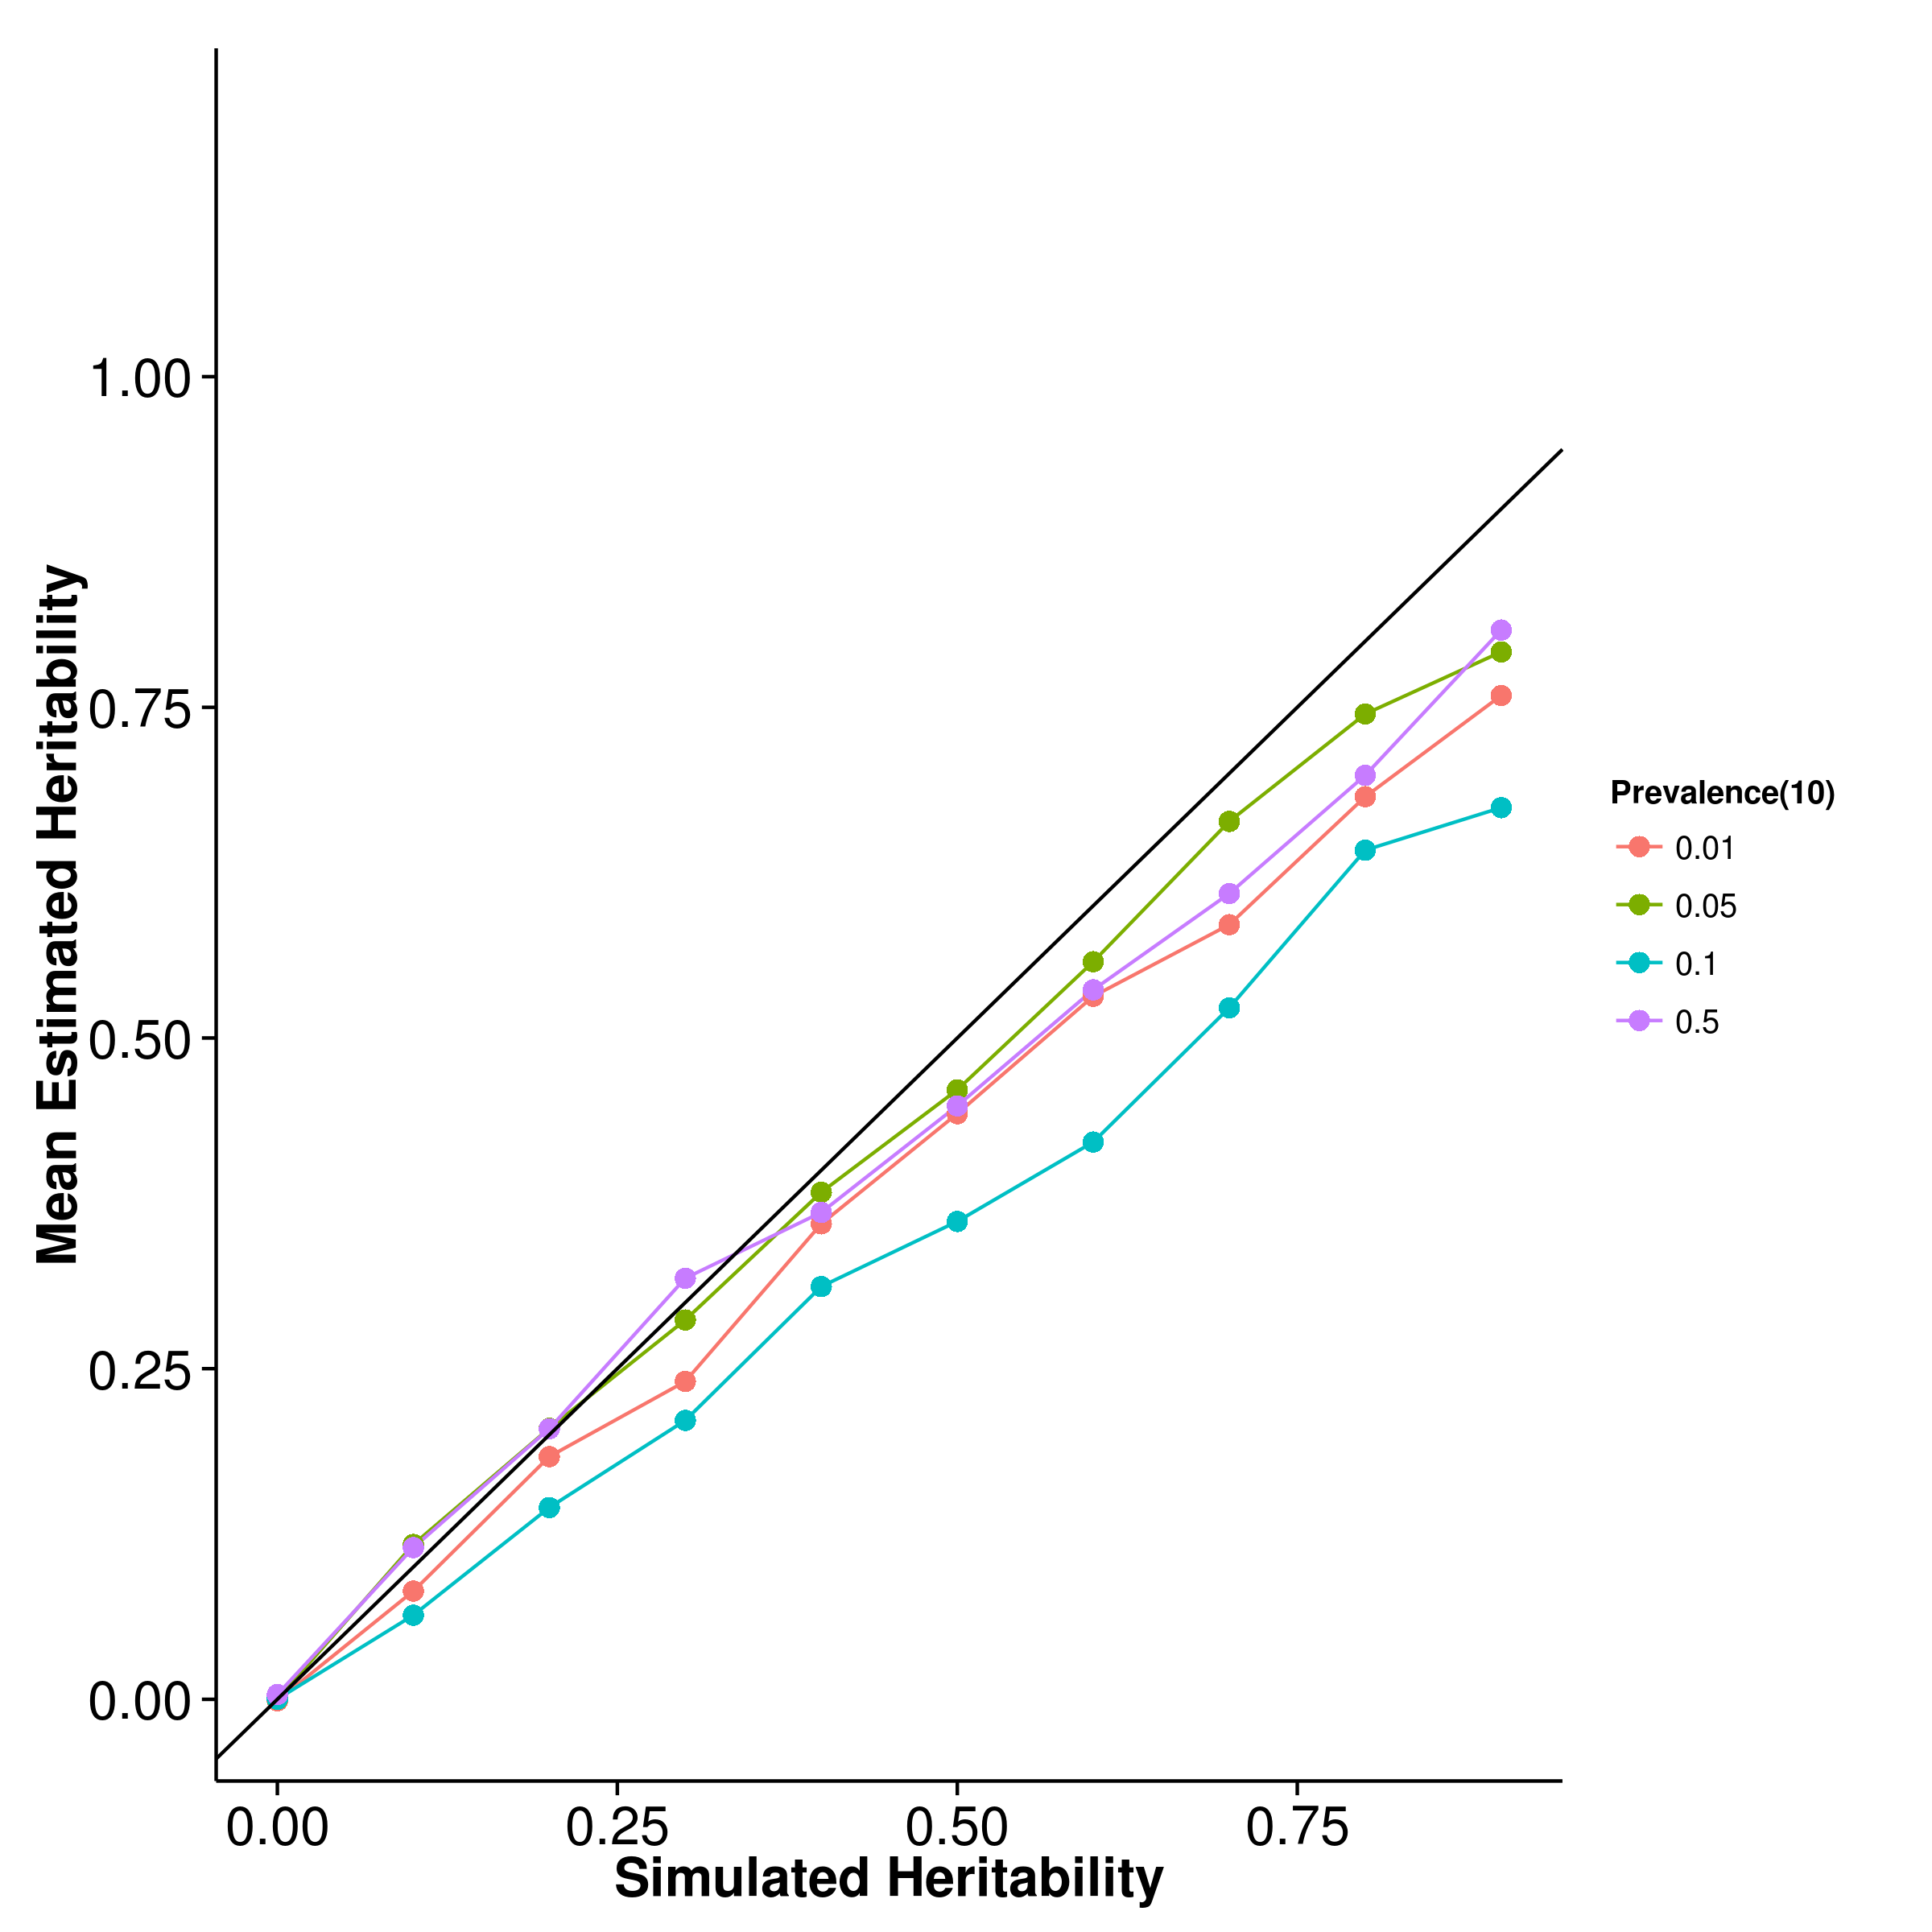
\includegraphics{figure/he_summary/cc_10c/ldscIn_CC_Rand_mean.png}}
				\label{fig:ldscInCC10RandMean}
			}
			\caption[Mean of Case Control Simulation Results (10 Causal)]
			{Mean of results from case control simulation with random effect size simulation with 10 causal \glspl{SNP}.
				The performance of \gls{gcta} was as suggested by \citet{Golan2014} where there was an underestimation as prevalence decreases.
				On the other hand, the upward bias of both \gls{ldsc} with fixed intercept and \gls{shrek} increases as the prevalence decreases whereas \gls{ldsc} with intercept estimation seems relatively robust to the change in prevalence.
				} 
			\label{fig:CC10RandMean}
		\end{figure}
		
		\begin{figure}
			\centering
			\subfloat[SHREK]{
				\scalebox{.4}{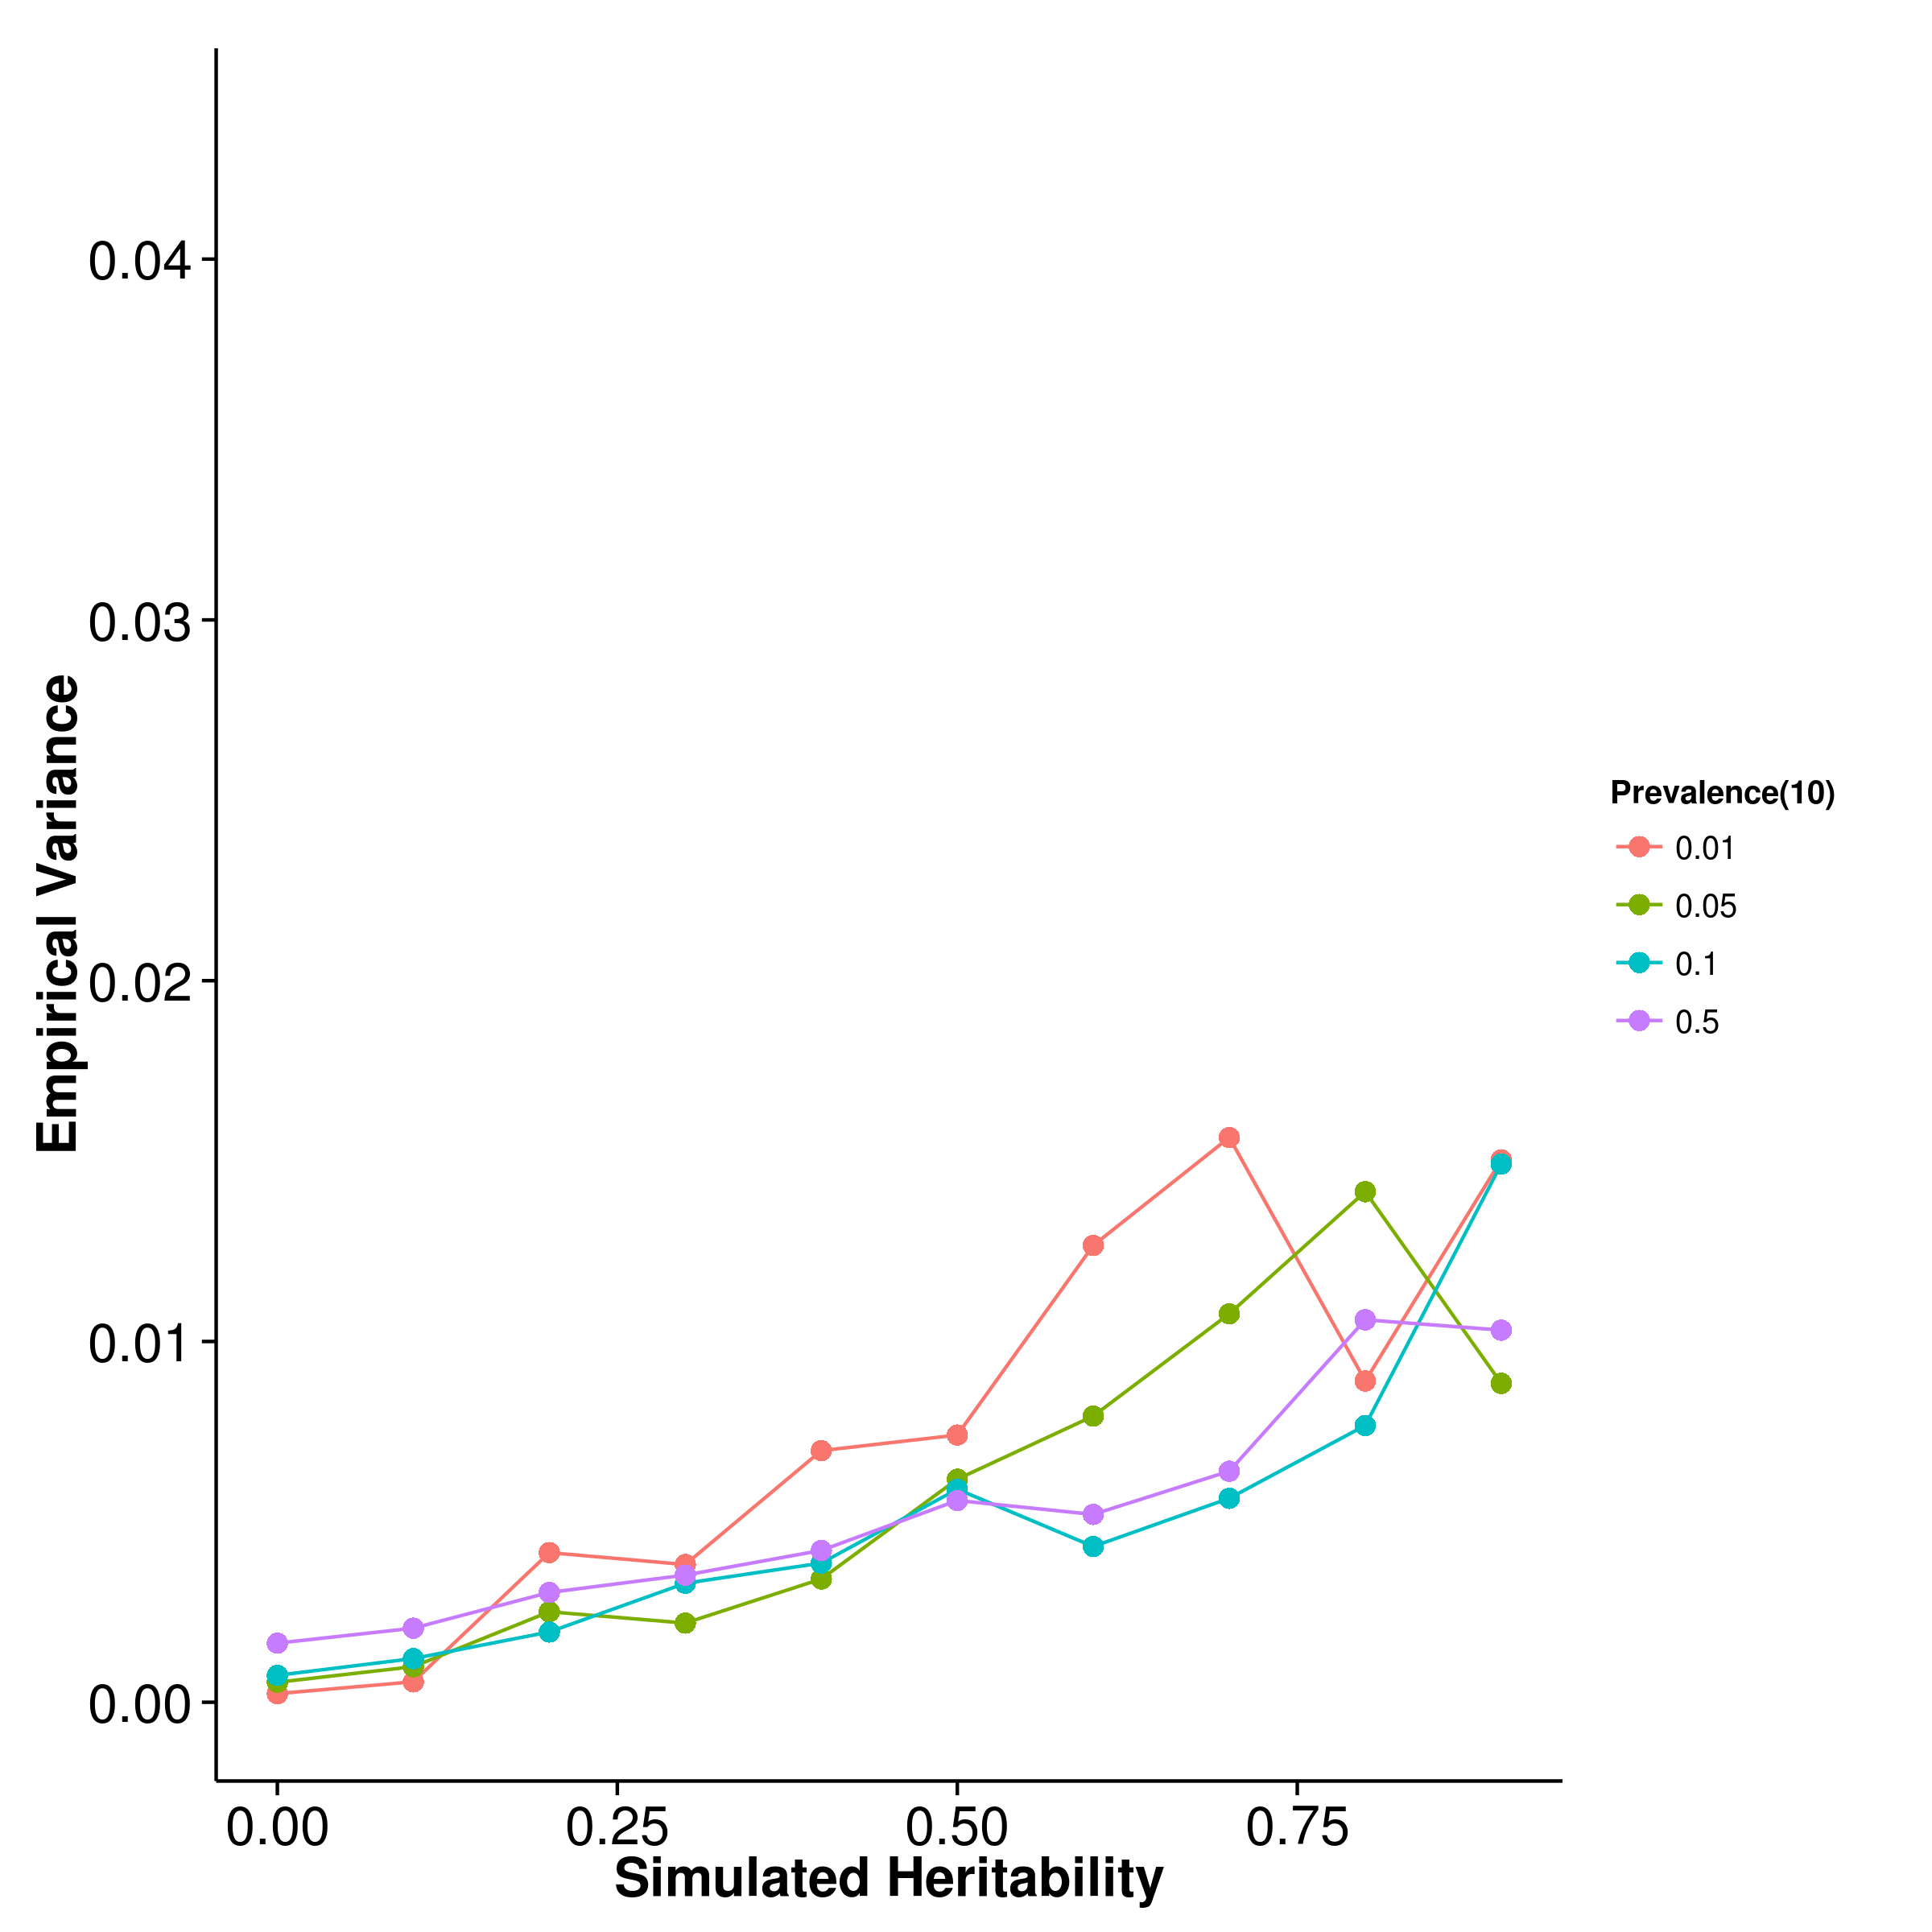
\includegraphics{figure/he_summary/cc_10c/shrek_CC_Rand_sd.png}}
				\label{fig:shrekCC10RandVar}
			}
			\subfloat[GCTA]{
				\scalebox{.4}{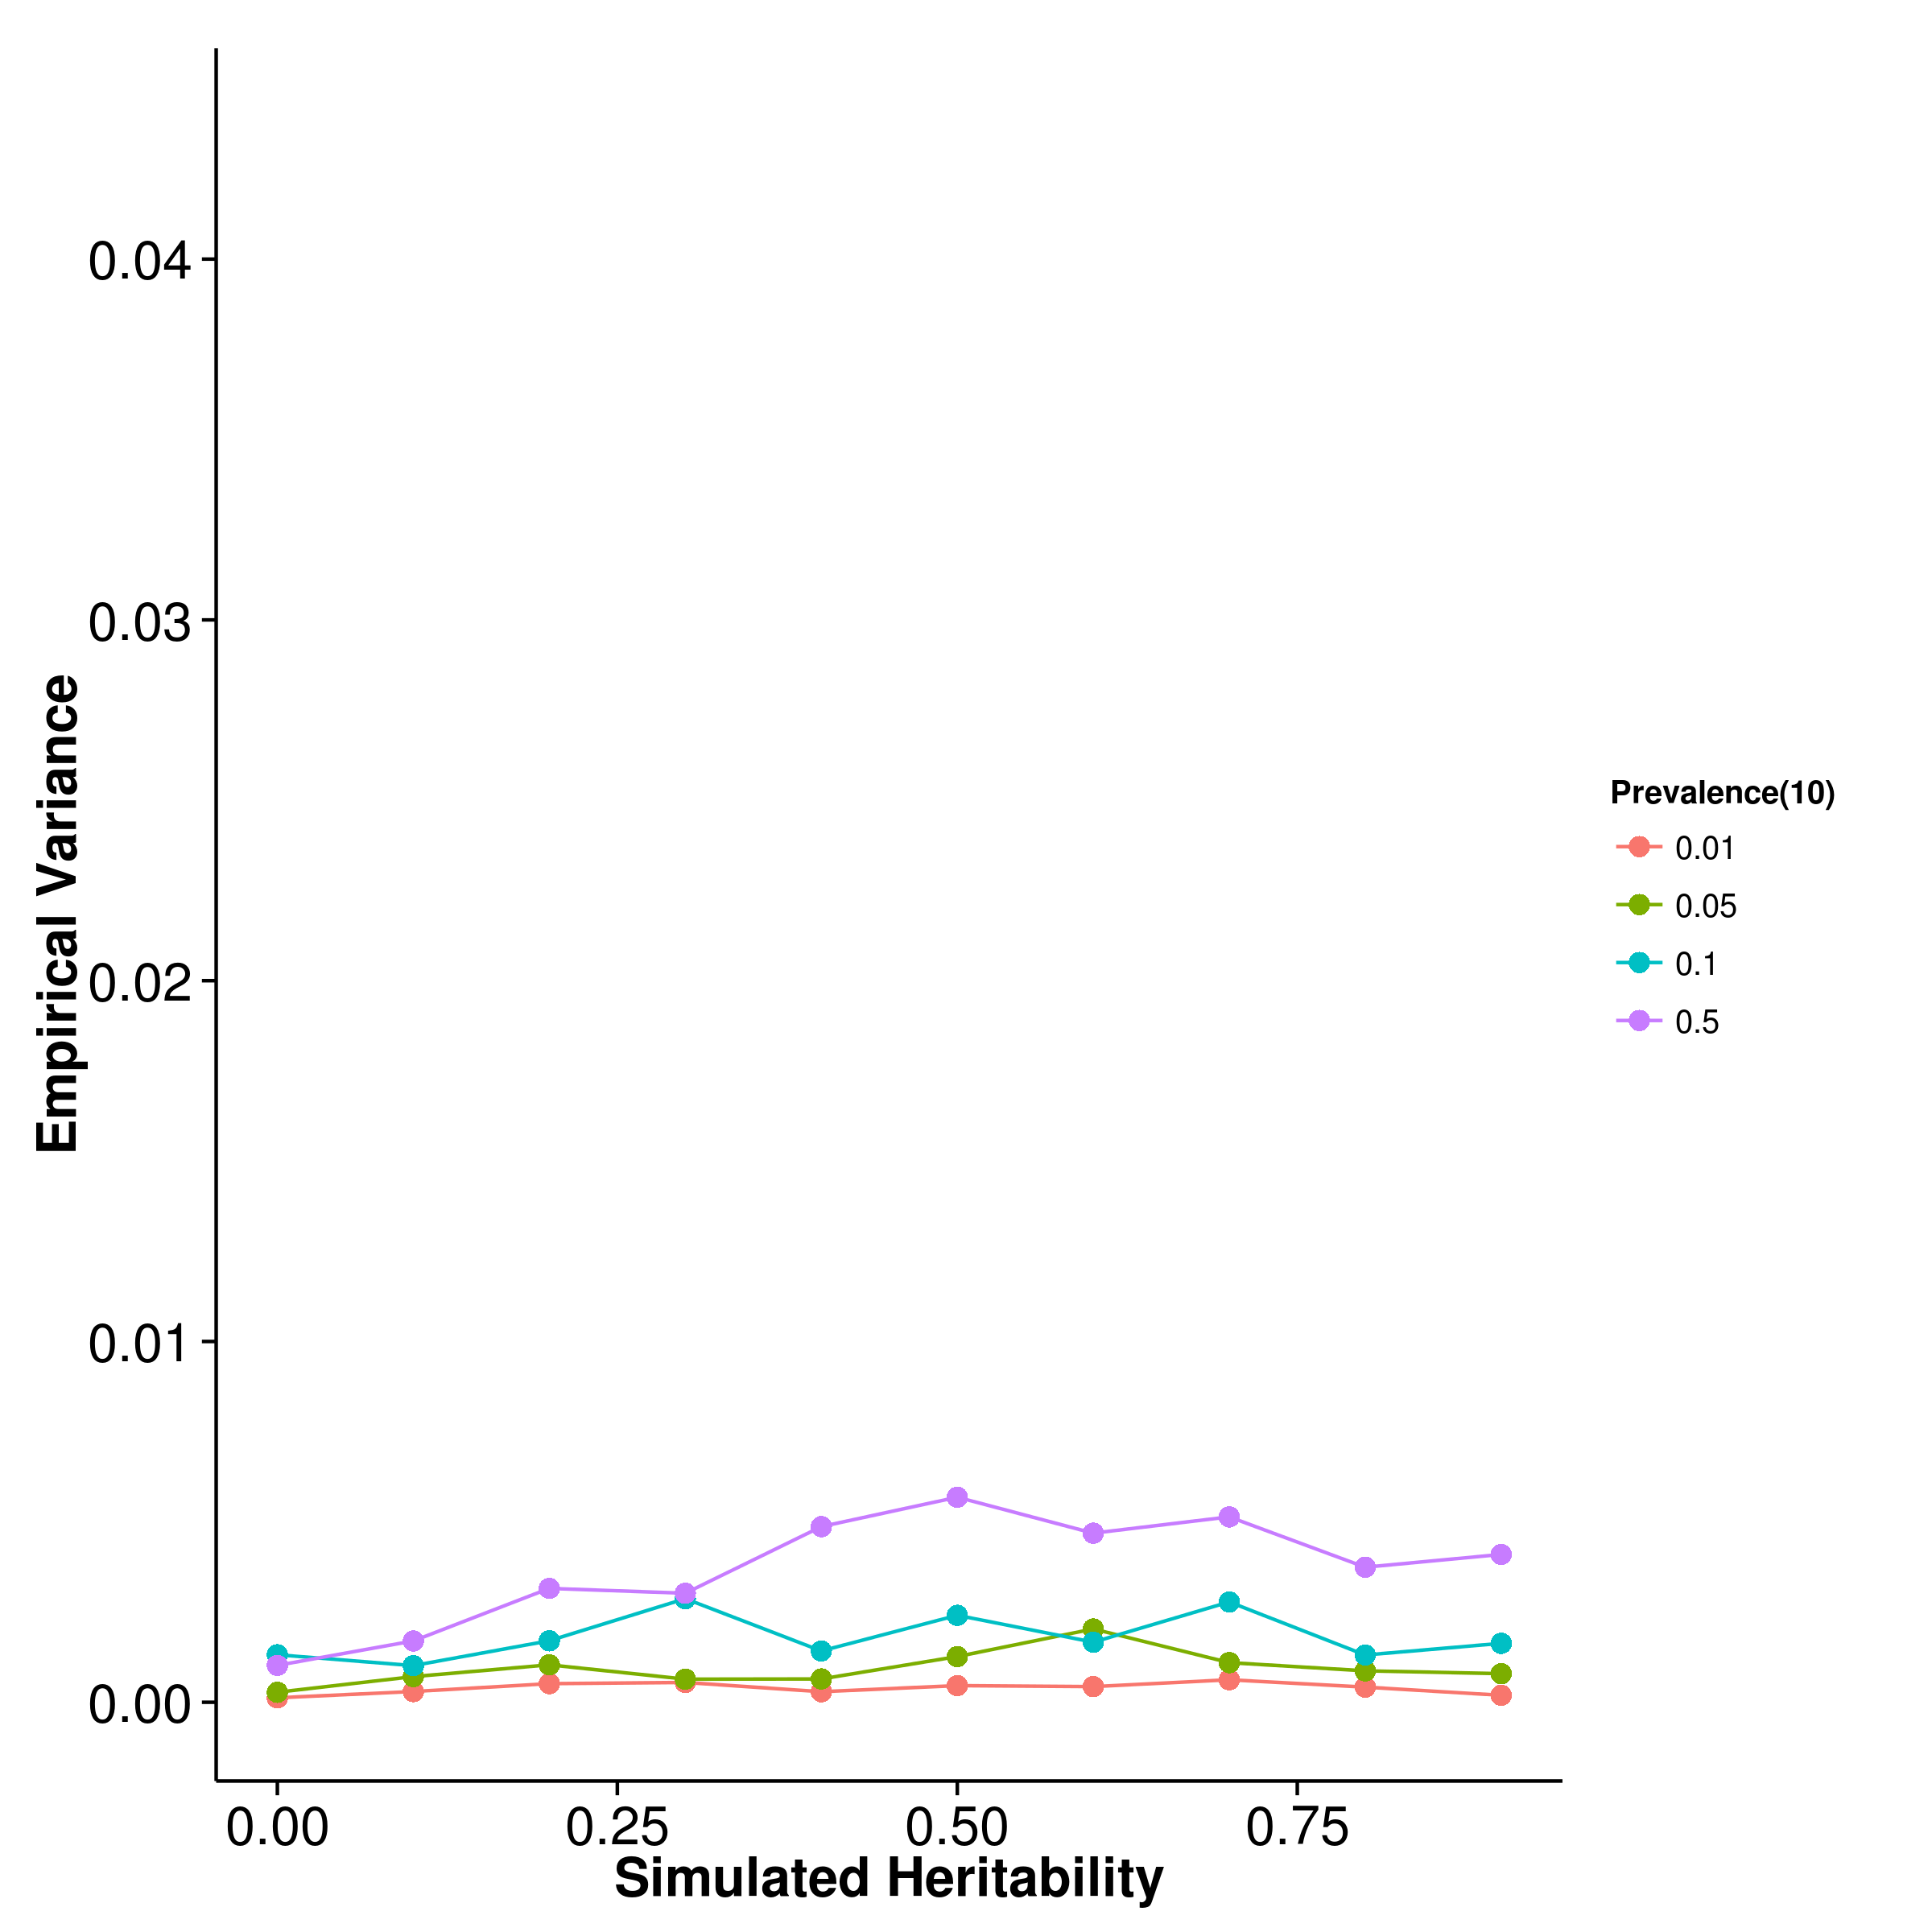
\includegraphics{figure/he_summary/cc_10c/gcta_CC_Rand_sd.png}}
				\label{fig:gctaCC10RandVar}
			}\\
			\subfloat[LDSC with fix intercept]{
				\scalebox{.4}{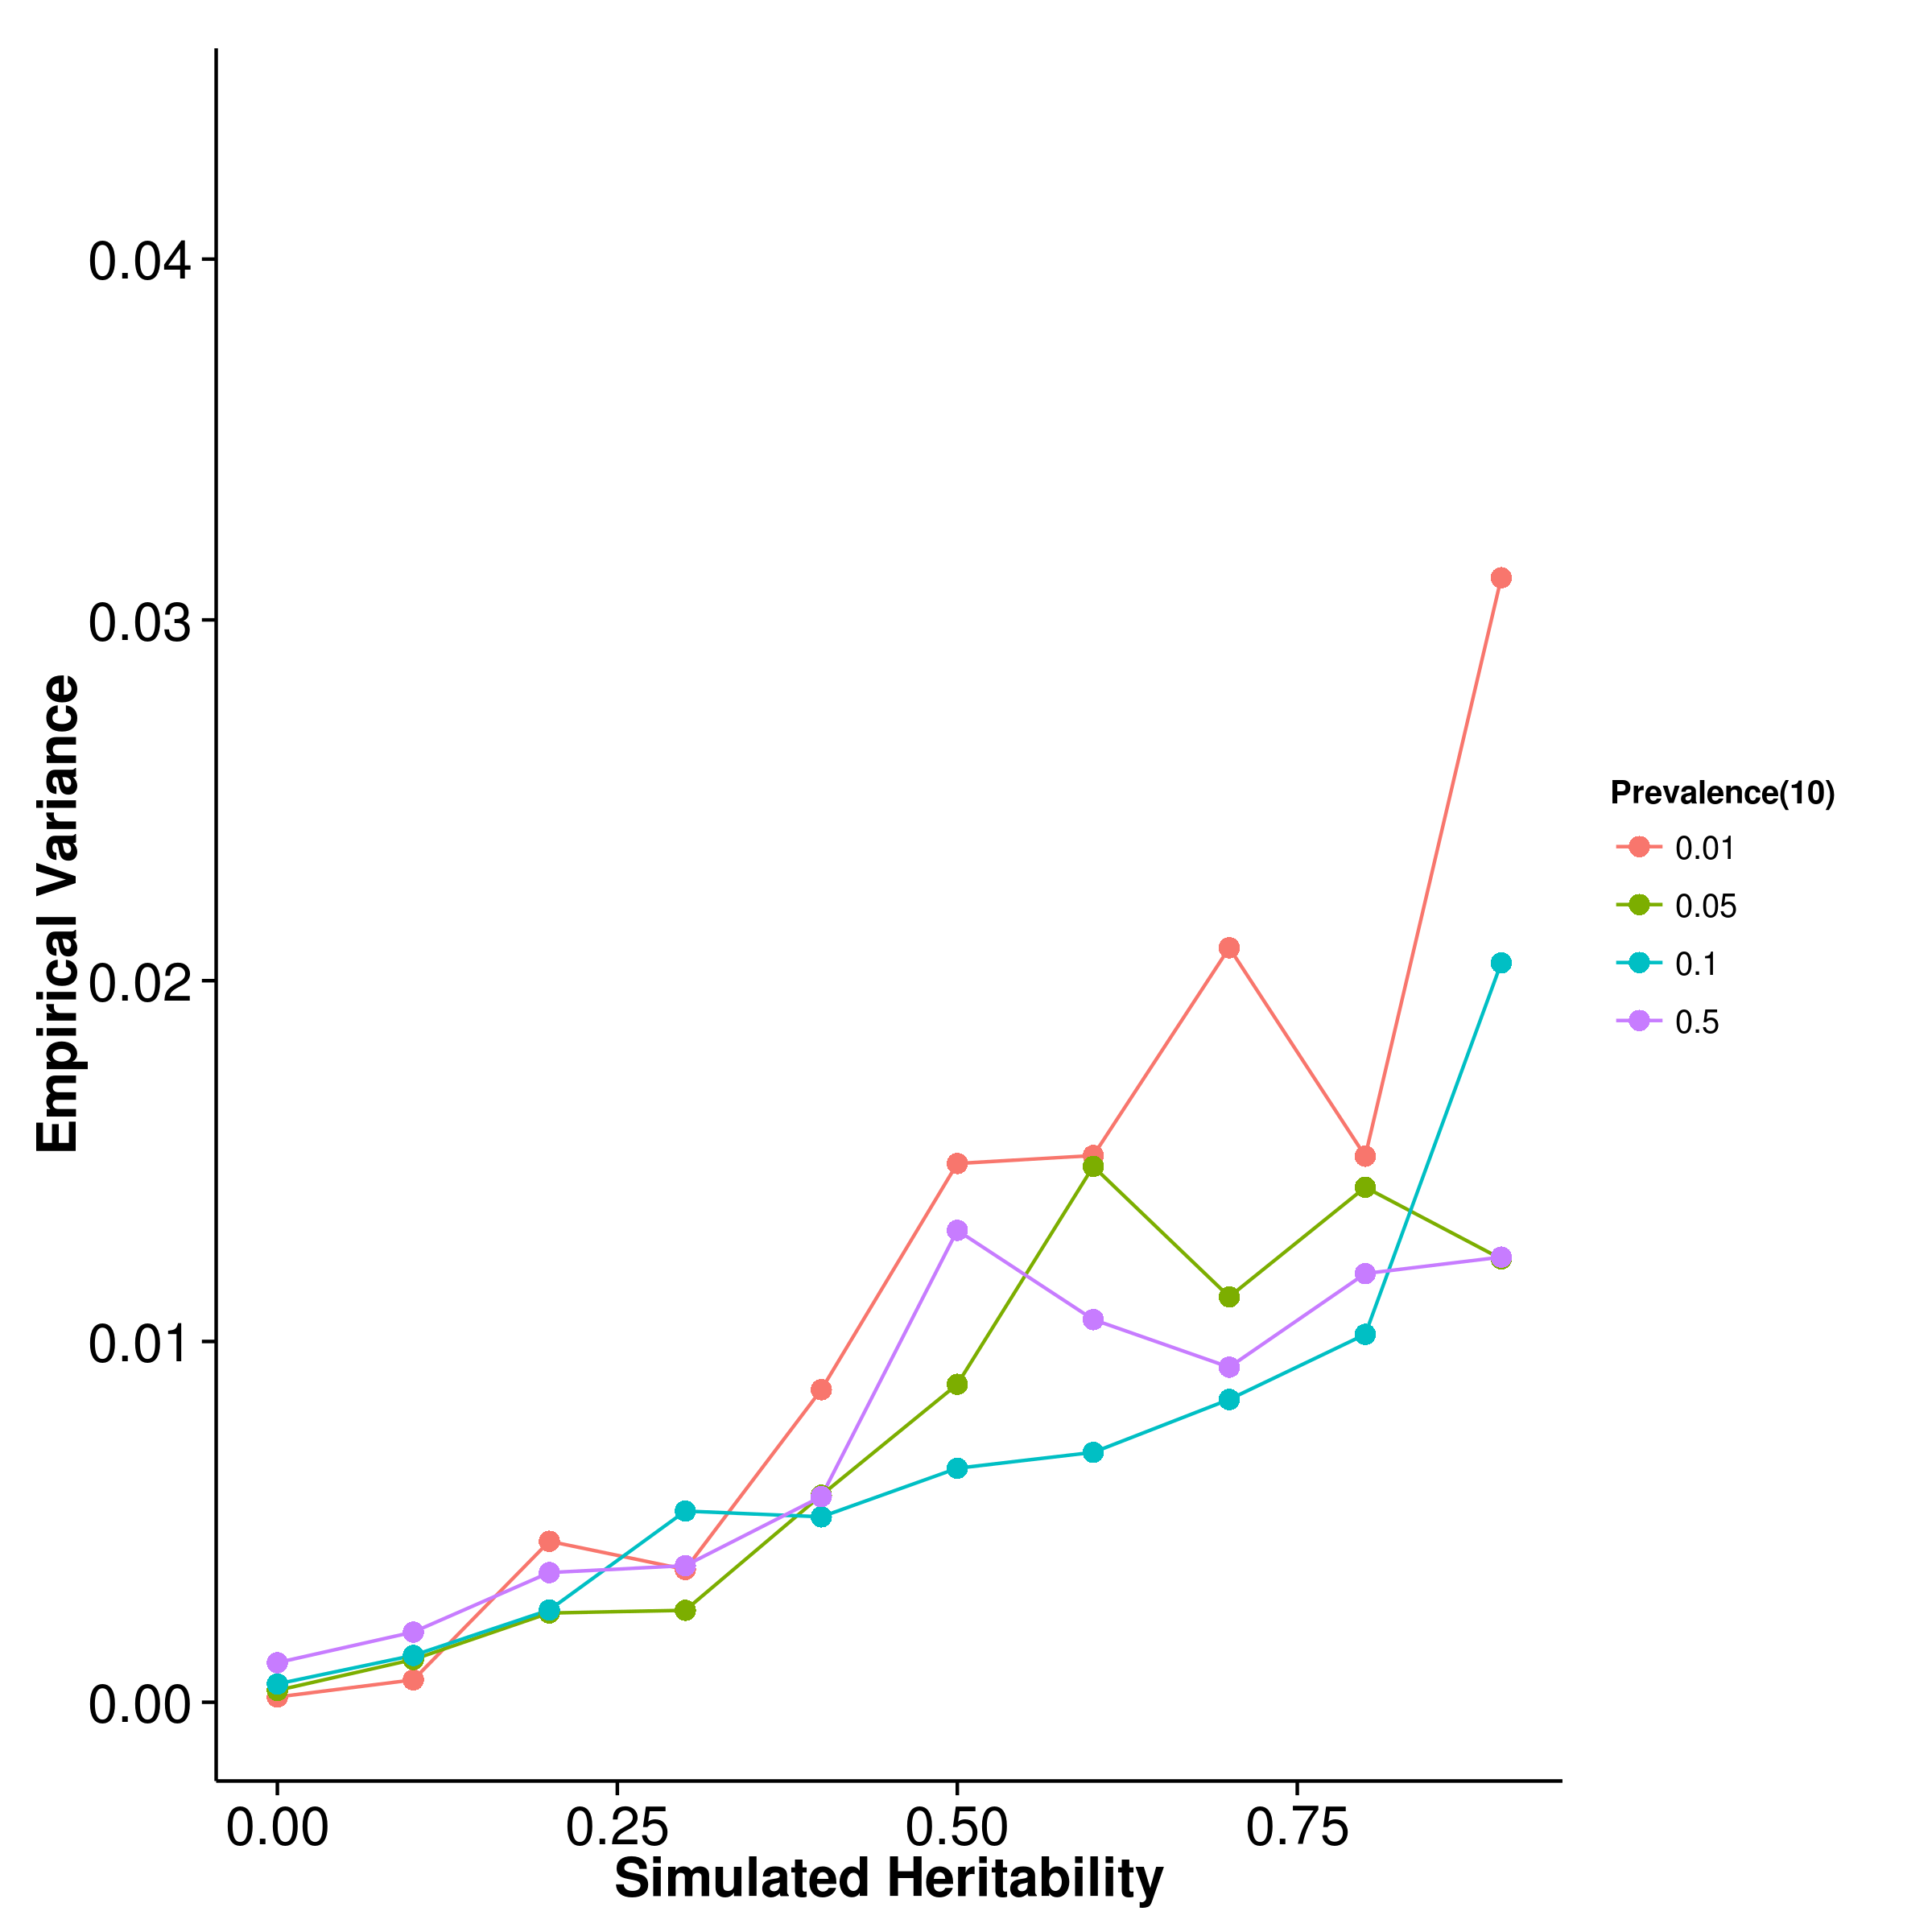
\includegraphics{figure/he_summary/cc_10c/ldsc_CC_Rand_sd.png}}
				\label{fig:ldscCC10RandVar}
			}
			\subfloat[LDSC with intercept estimation]{
				
				\scalebox{.4}{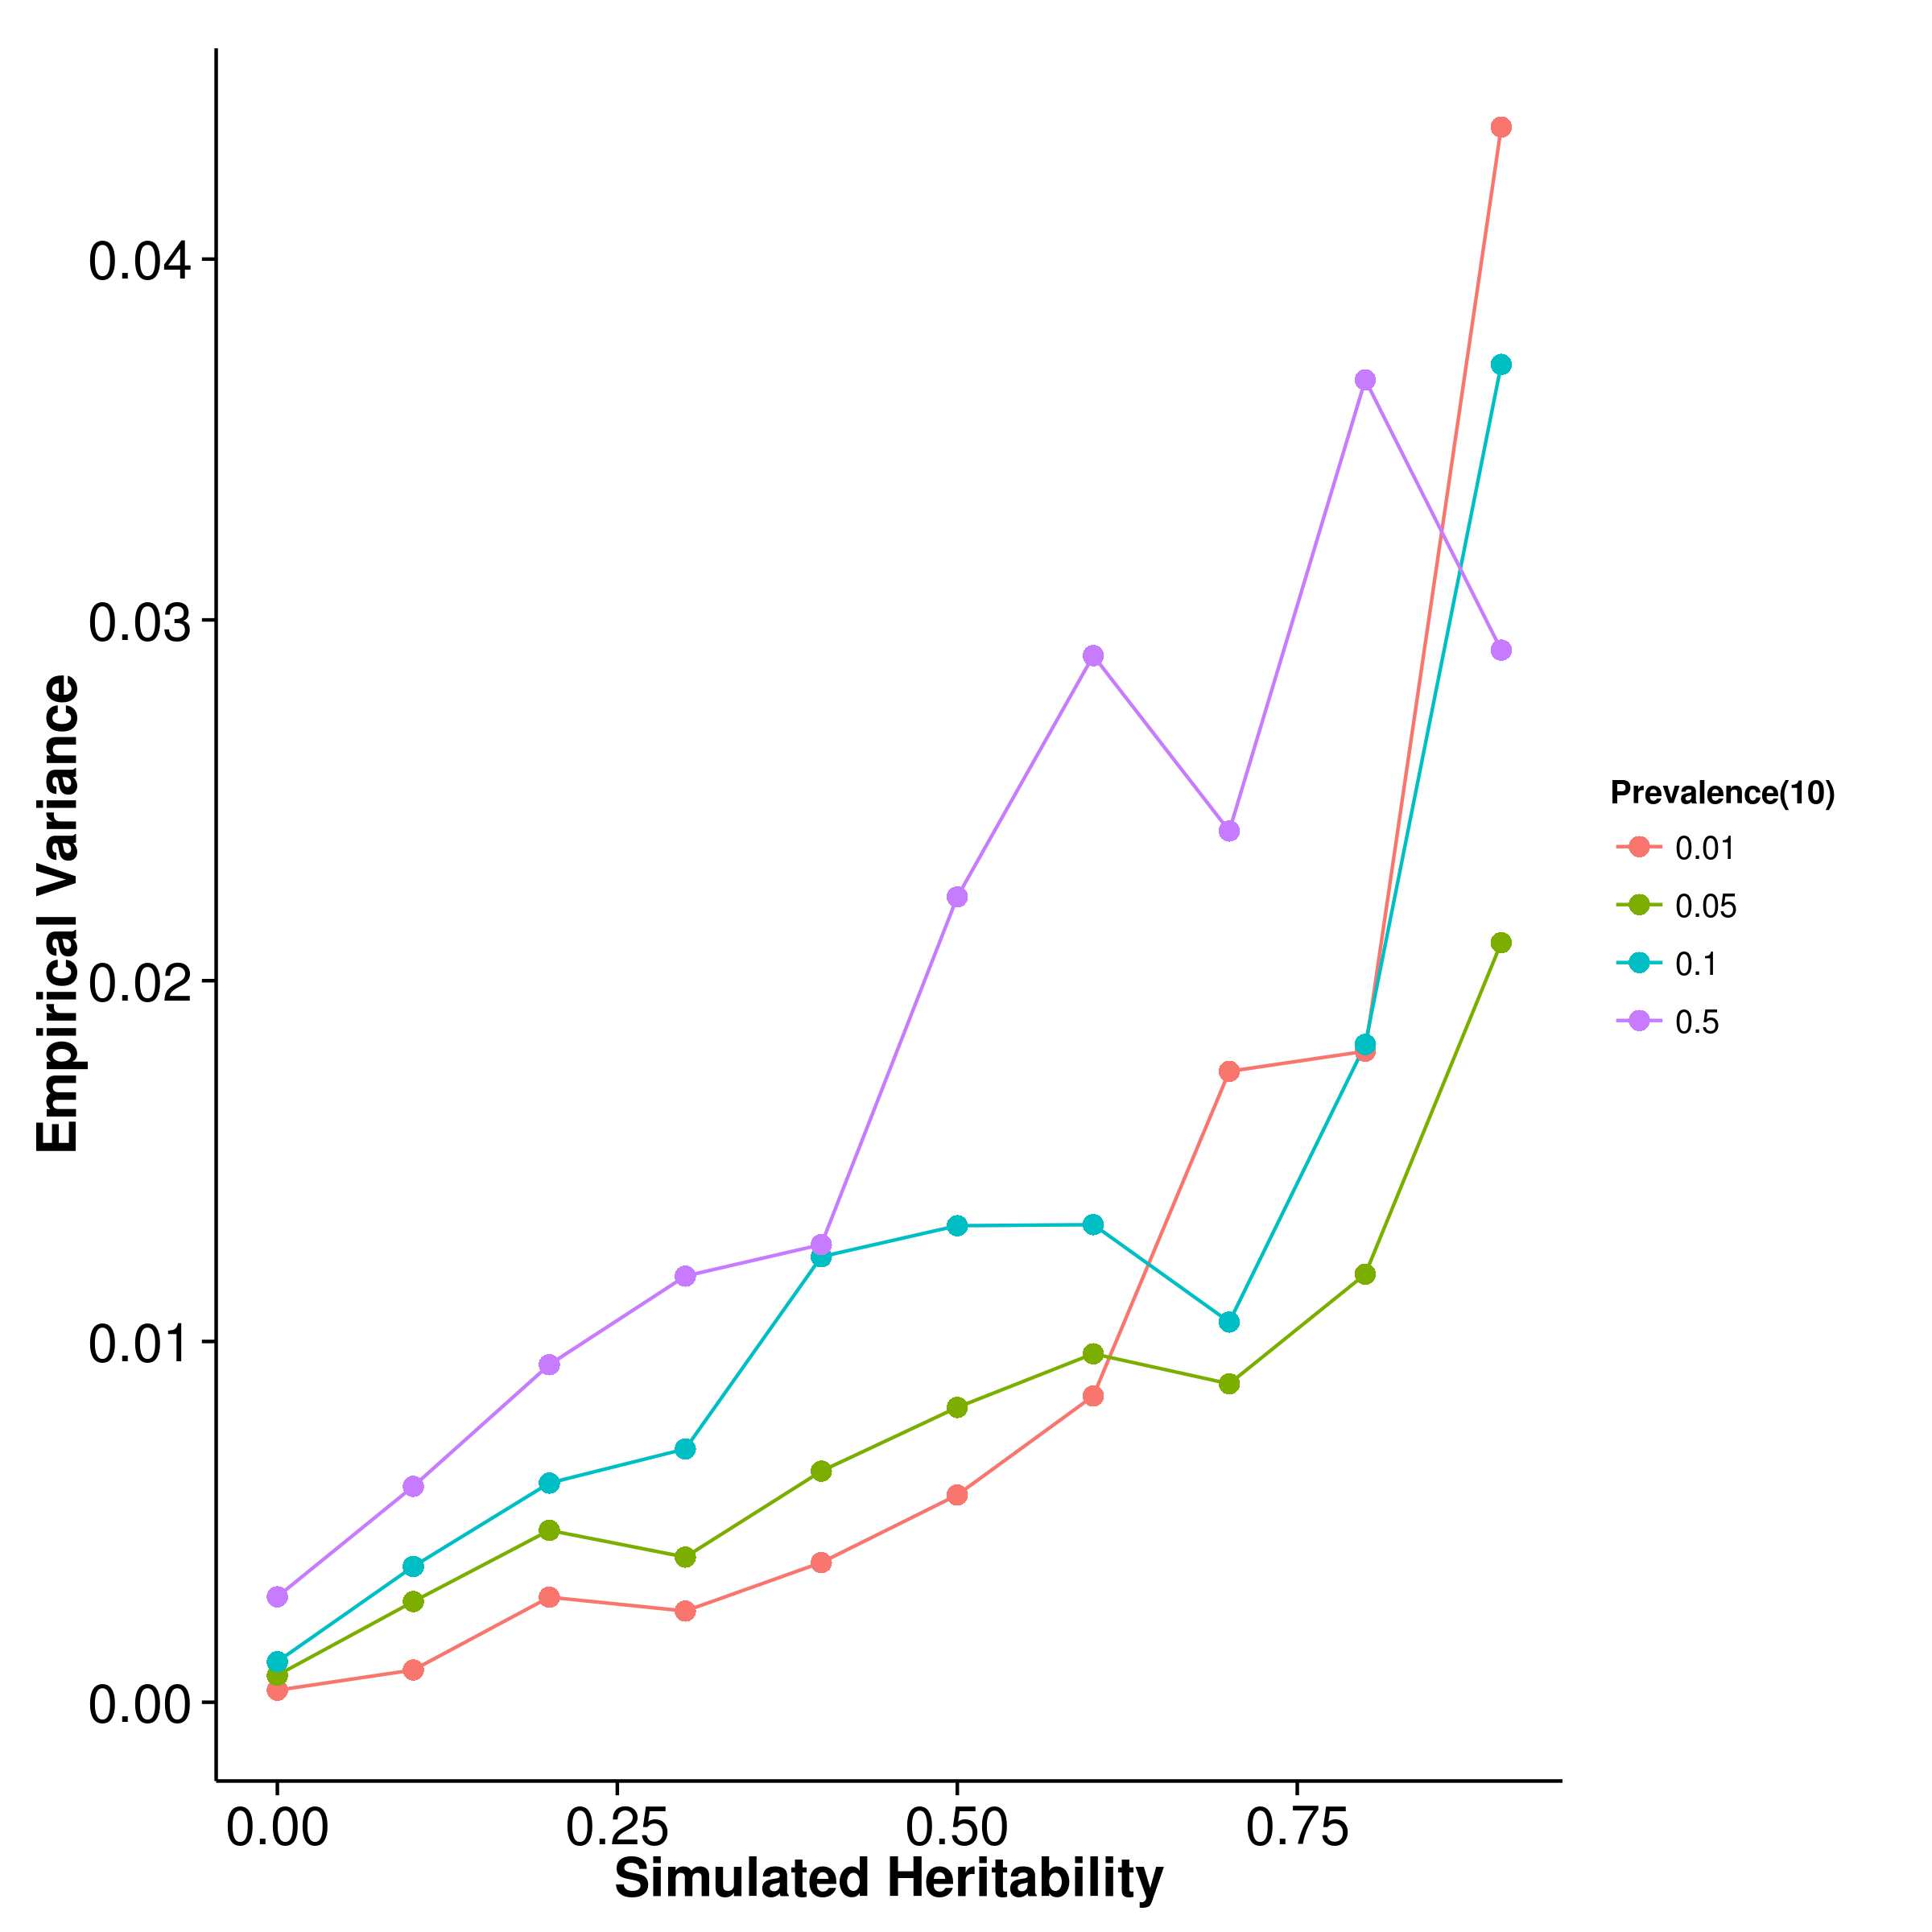
\includegraphics{figure/he_summary/cc_10c/ldscIn_CC_Rand_sd.png}}
				\label{fig:ldscInCC10RandVar}
			}
			\caption[Variance of Case Control Simulation Results (10 Causal)]
			{Variance of results from case control simulation with random effect size simulation with 10 causal \glspl{SNP}.
				There were no clear pattern as to how the prevalence affect the empirical variance of estimates from \gls{shrek} and \gls{ldsc}. 
				For \gls{gcta}, it seems like a larger prevalence tends to result in a larger empirical variance. 
				Again, \gls{gcta} has the lowest variance, follow by \gls{shrek} and \gls{ldsc} with fixed intercept.
				Nonetheless, it was important to remember that in case control simulation, a much smaller amount of \glspl{SNP} was used, thus the results was not directly comparable to results from the quantitative simulation.
			} 
			\label{fig:CC10RandVar}
		\end{figure}
		
		
		\begin{figure}
			\centering
			\subfloat[SHREK]{
				\scalebox{.4}{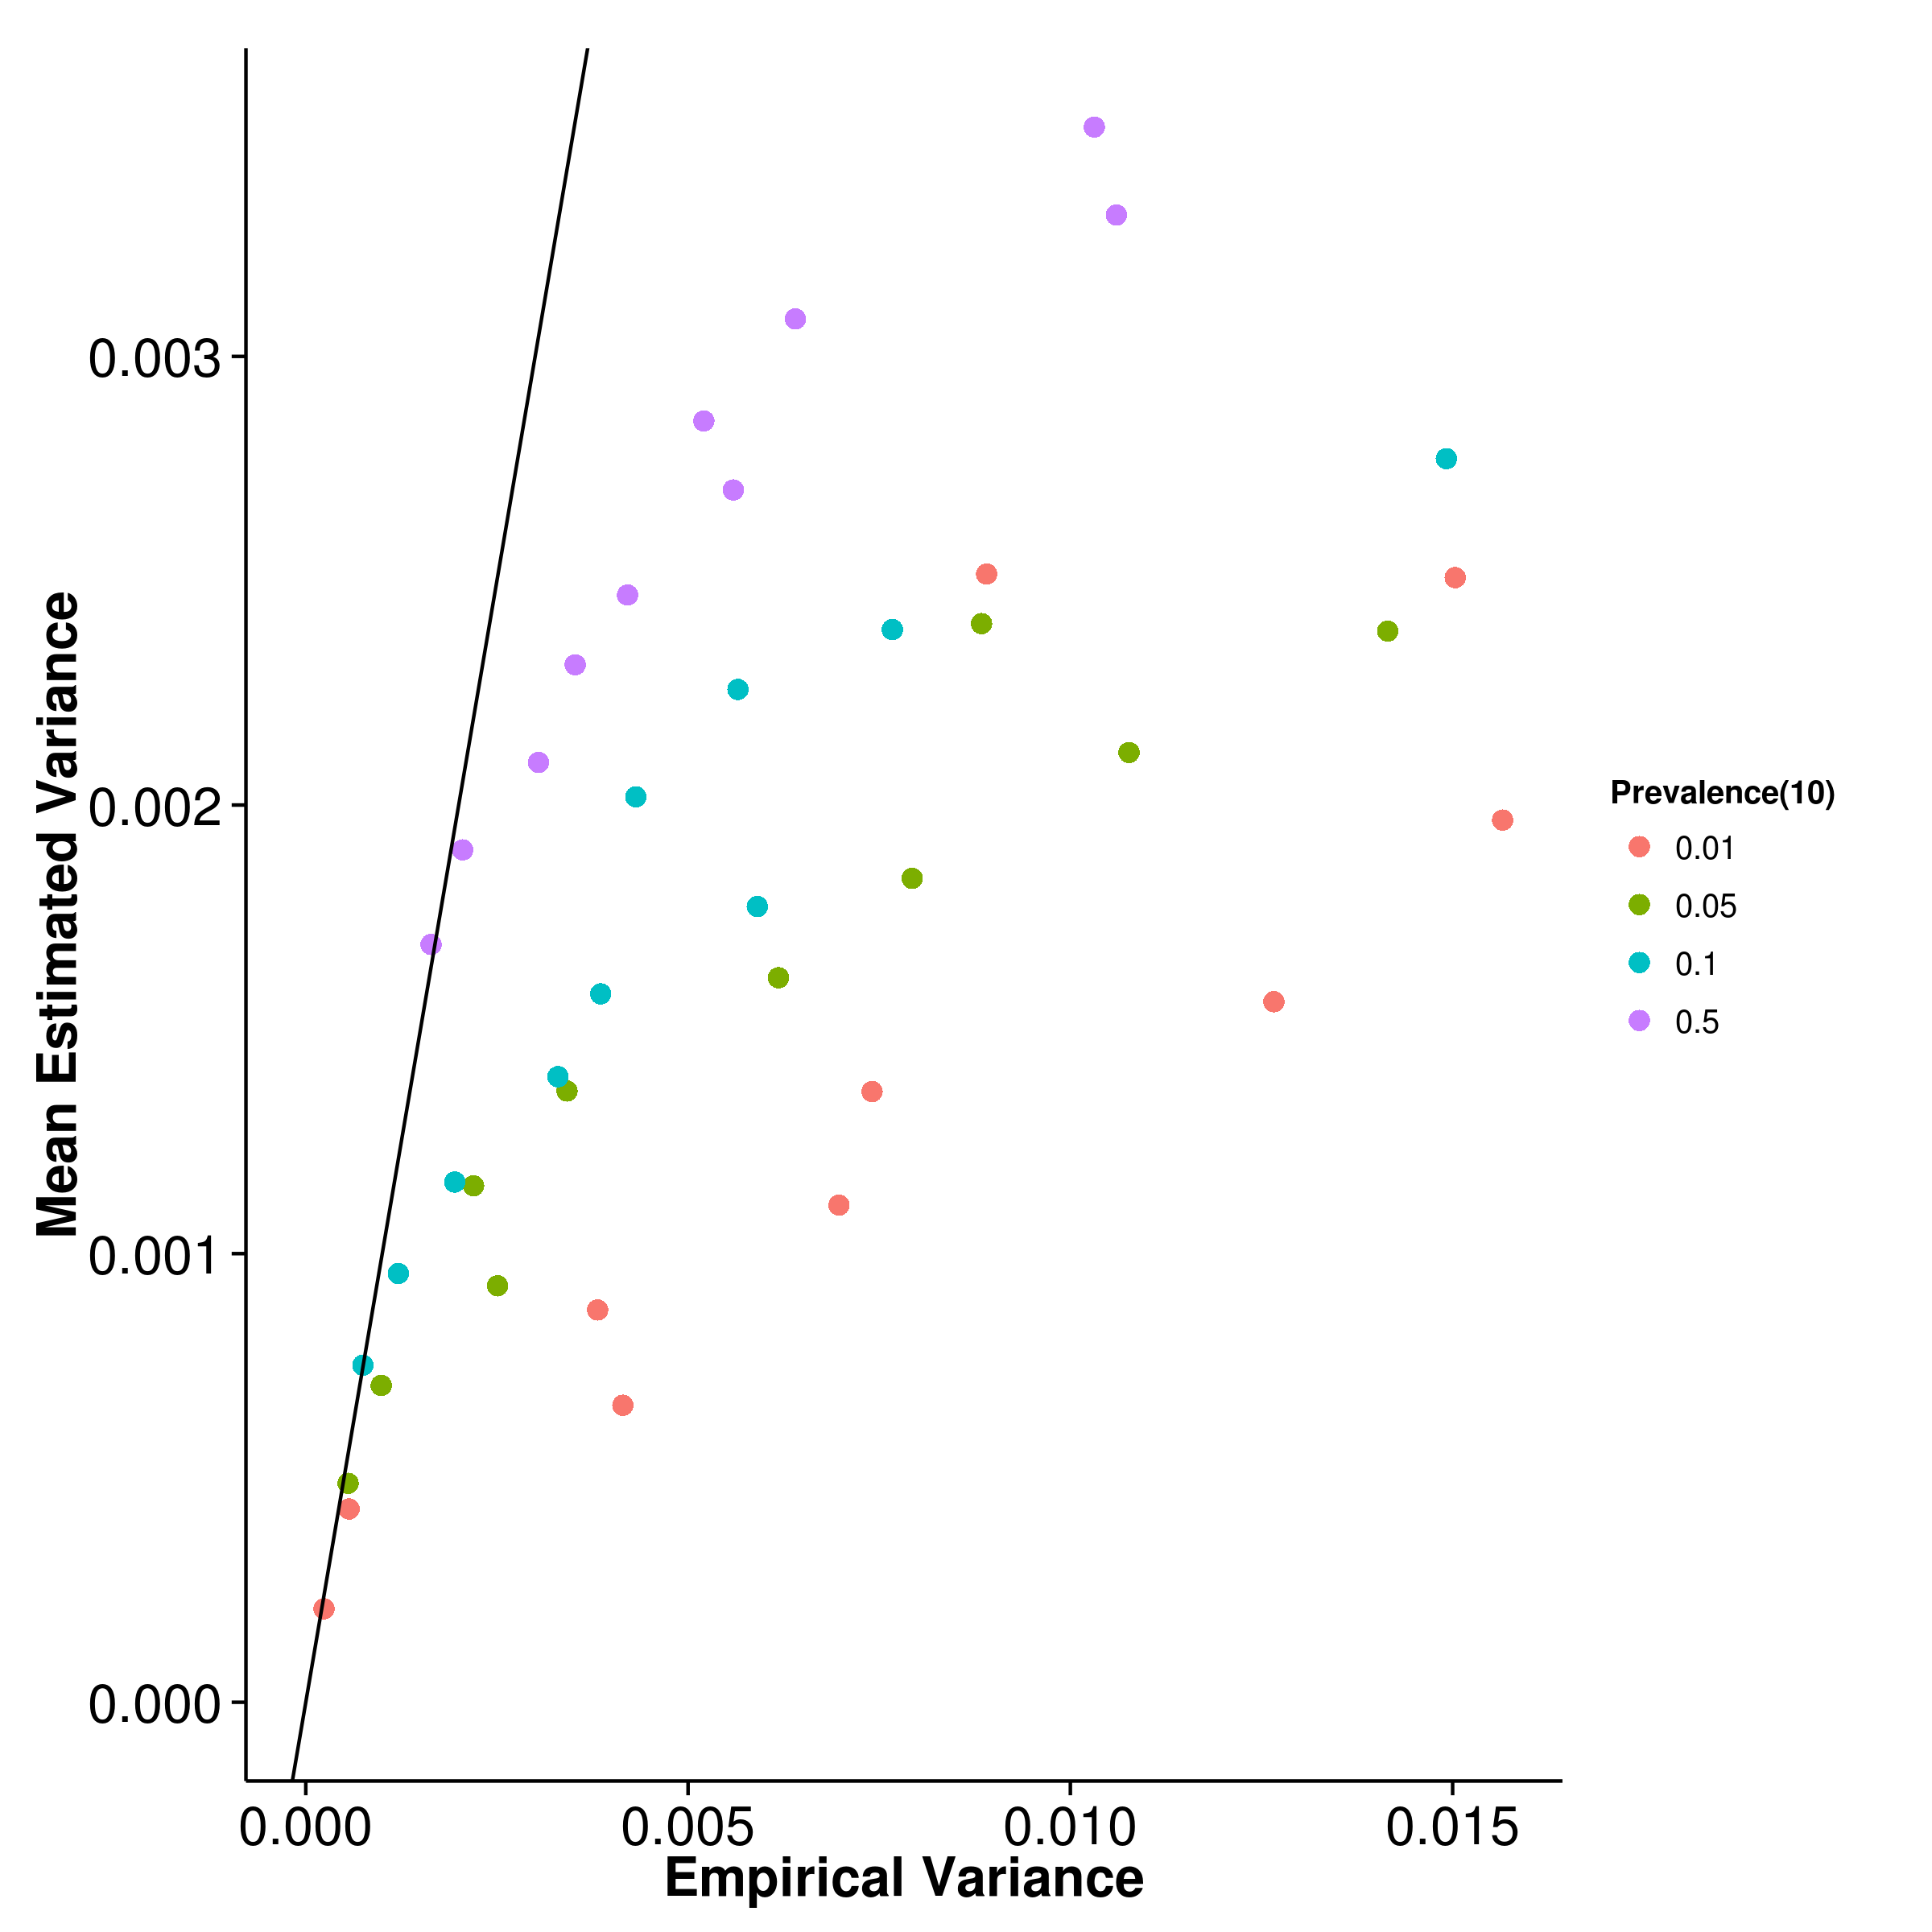
\includegraphics{figure/he_summary/cc_10c/shrek_CC_Rand_sdCom.png}}
				\label{fig:shrekCC10RandVarCom}
			}
			\subfloat[GCTA]{
				\scalebox{.4}{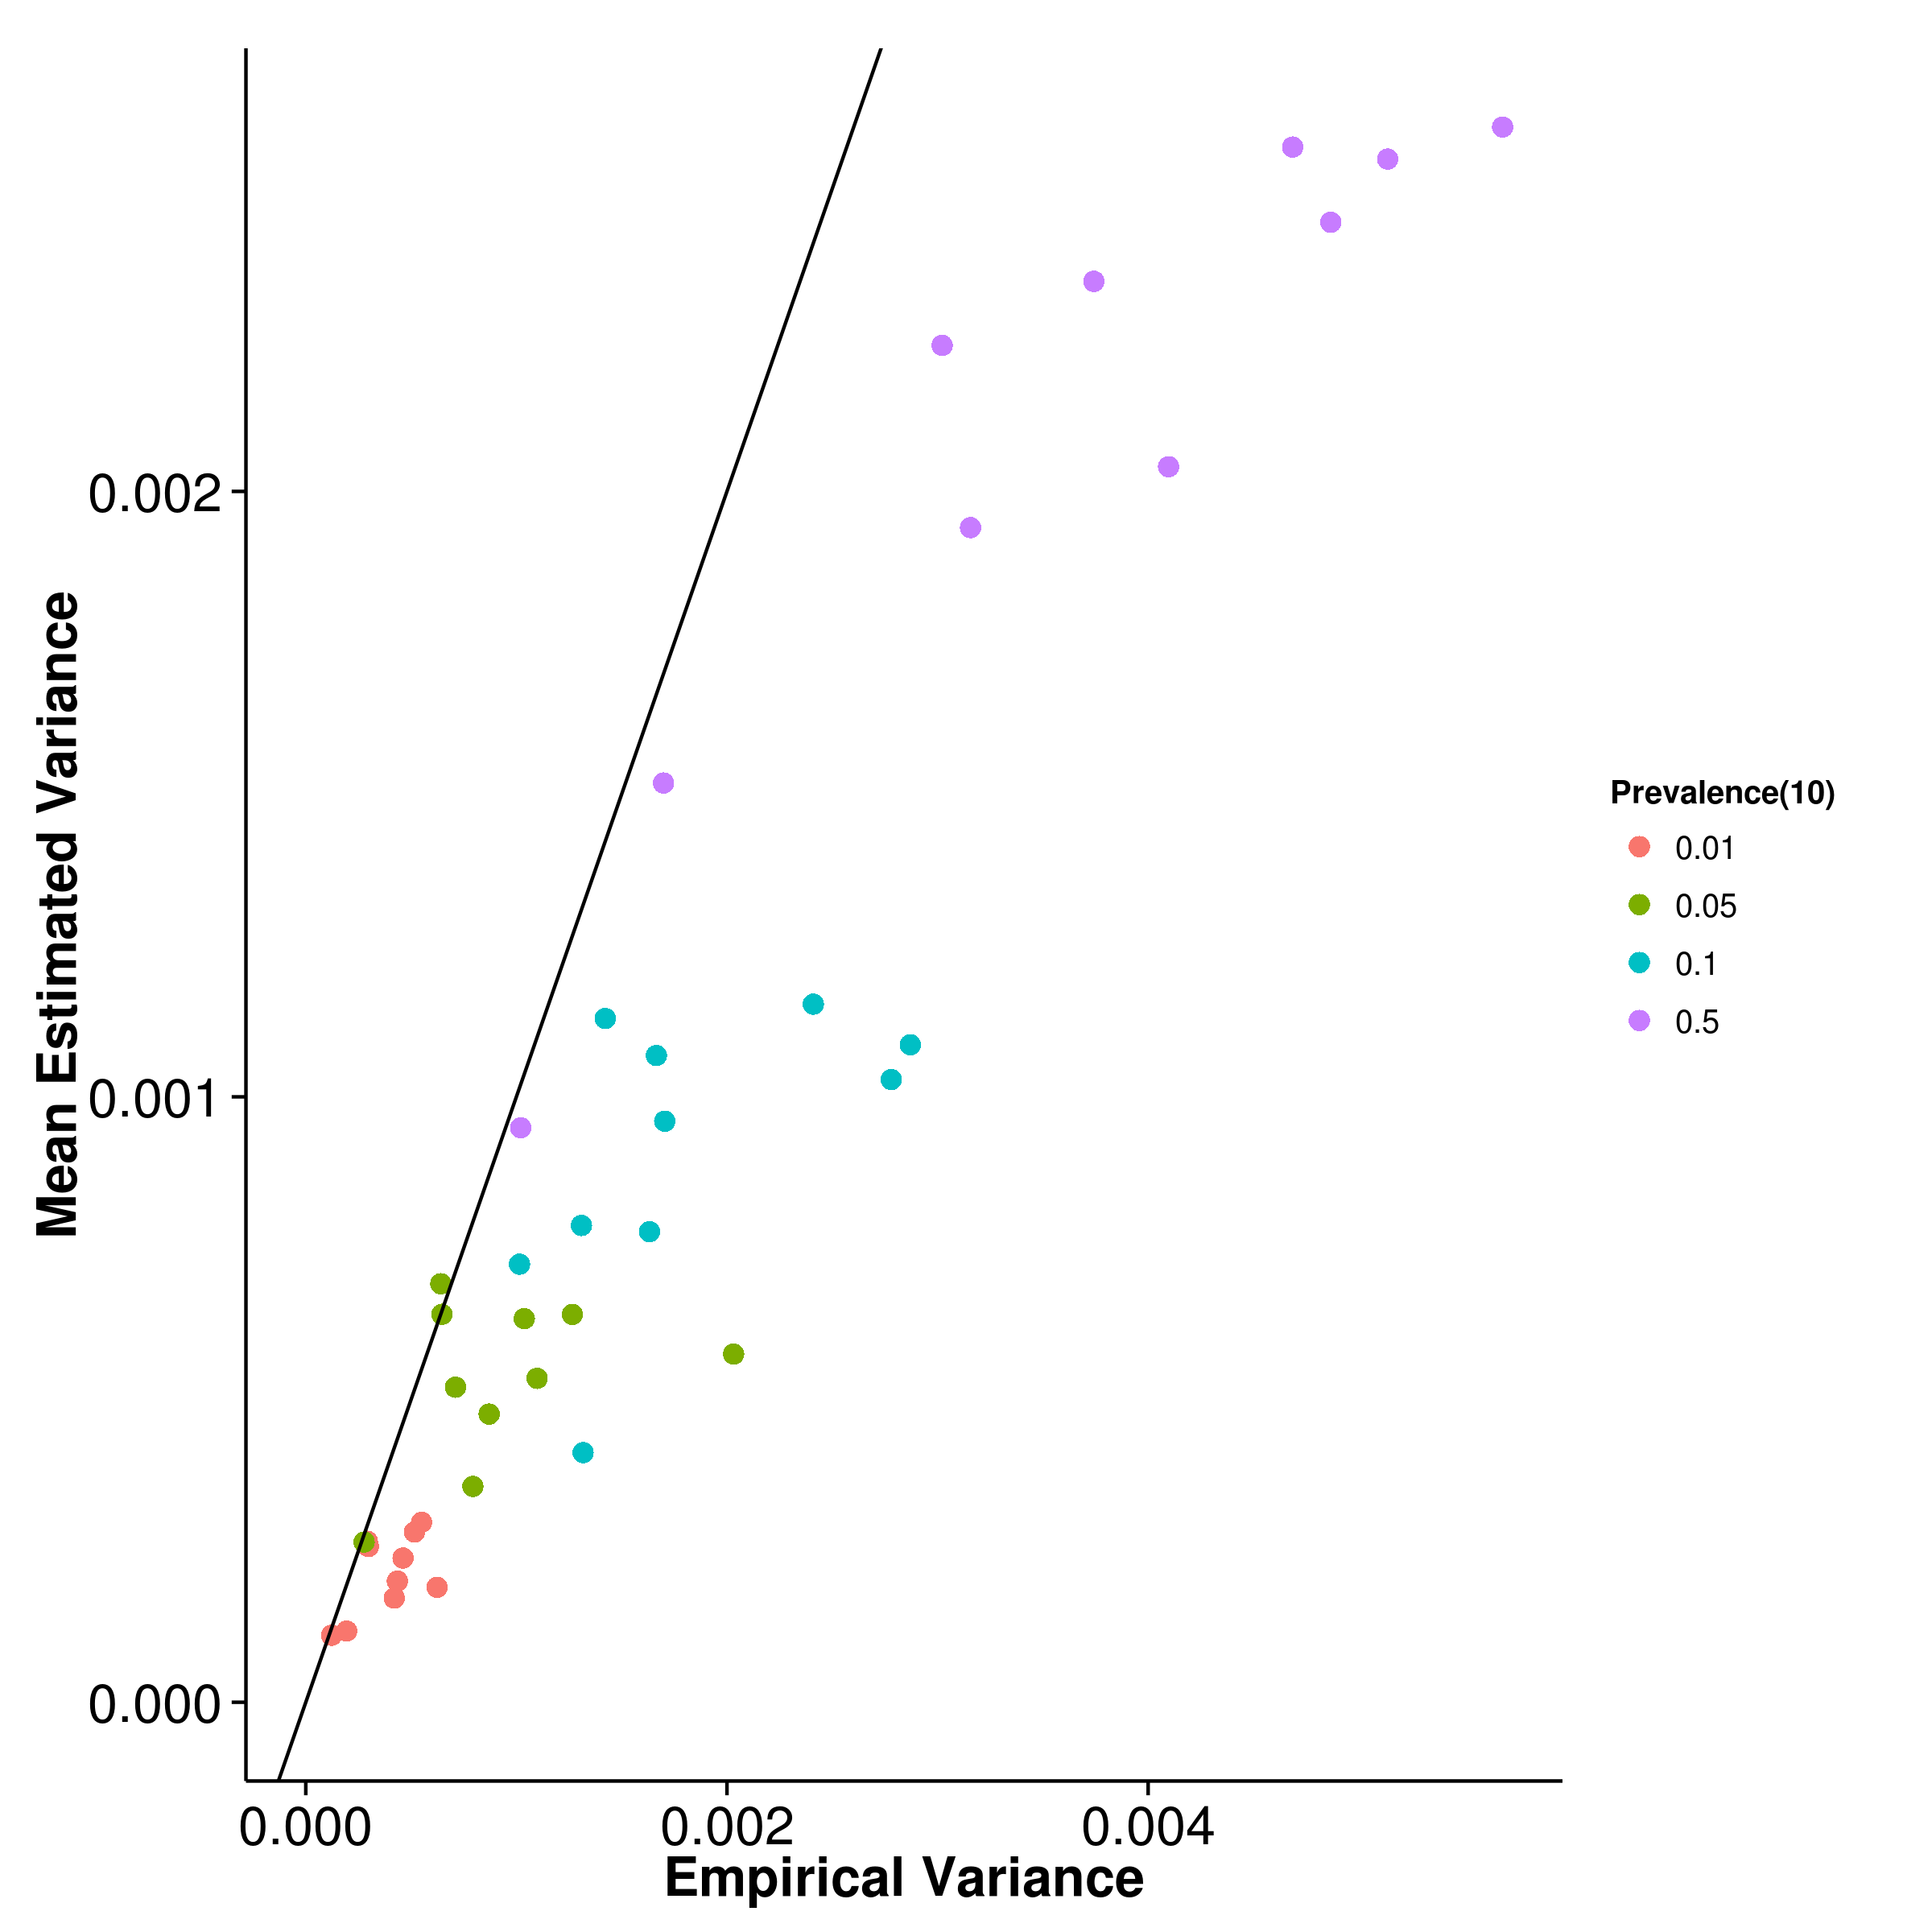
\includegraphics{figure/he_summary/cc_10c/gcta_CC_Rand_sdCom.png}}
				\label{fig:gctaCC10RandVarCom}
			}\\
			\subfloat[LDSC with fix intercept]{
				\scalebox{.4}{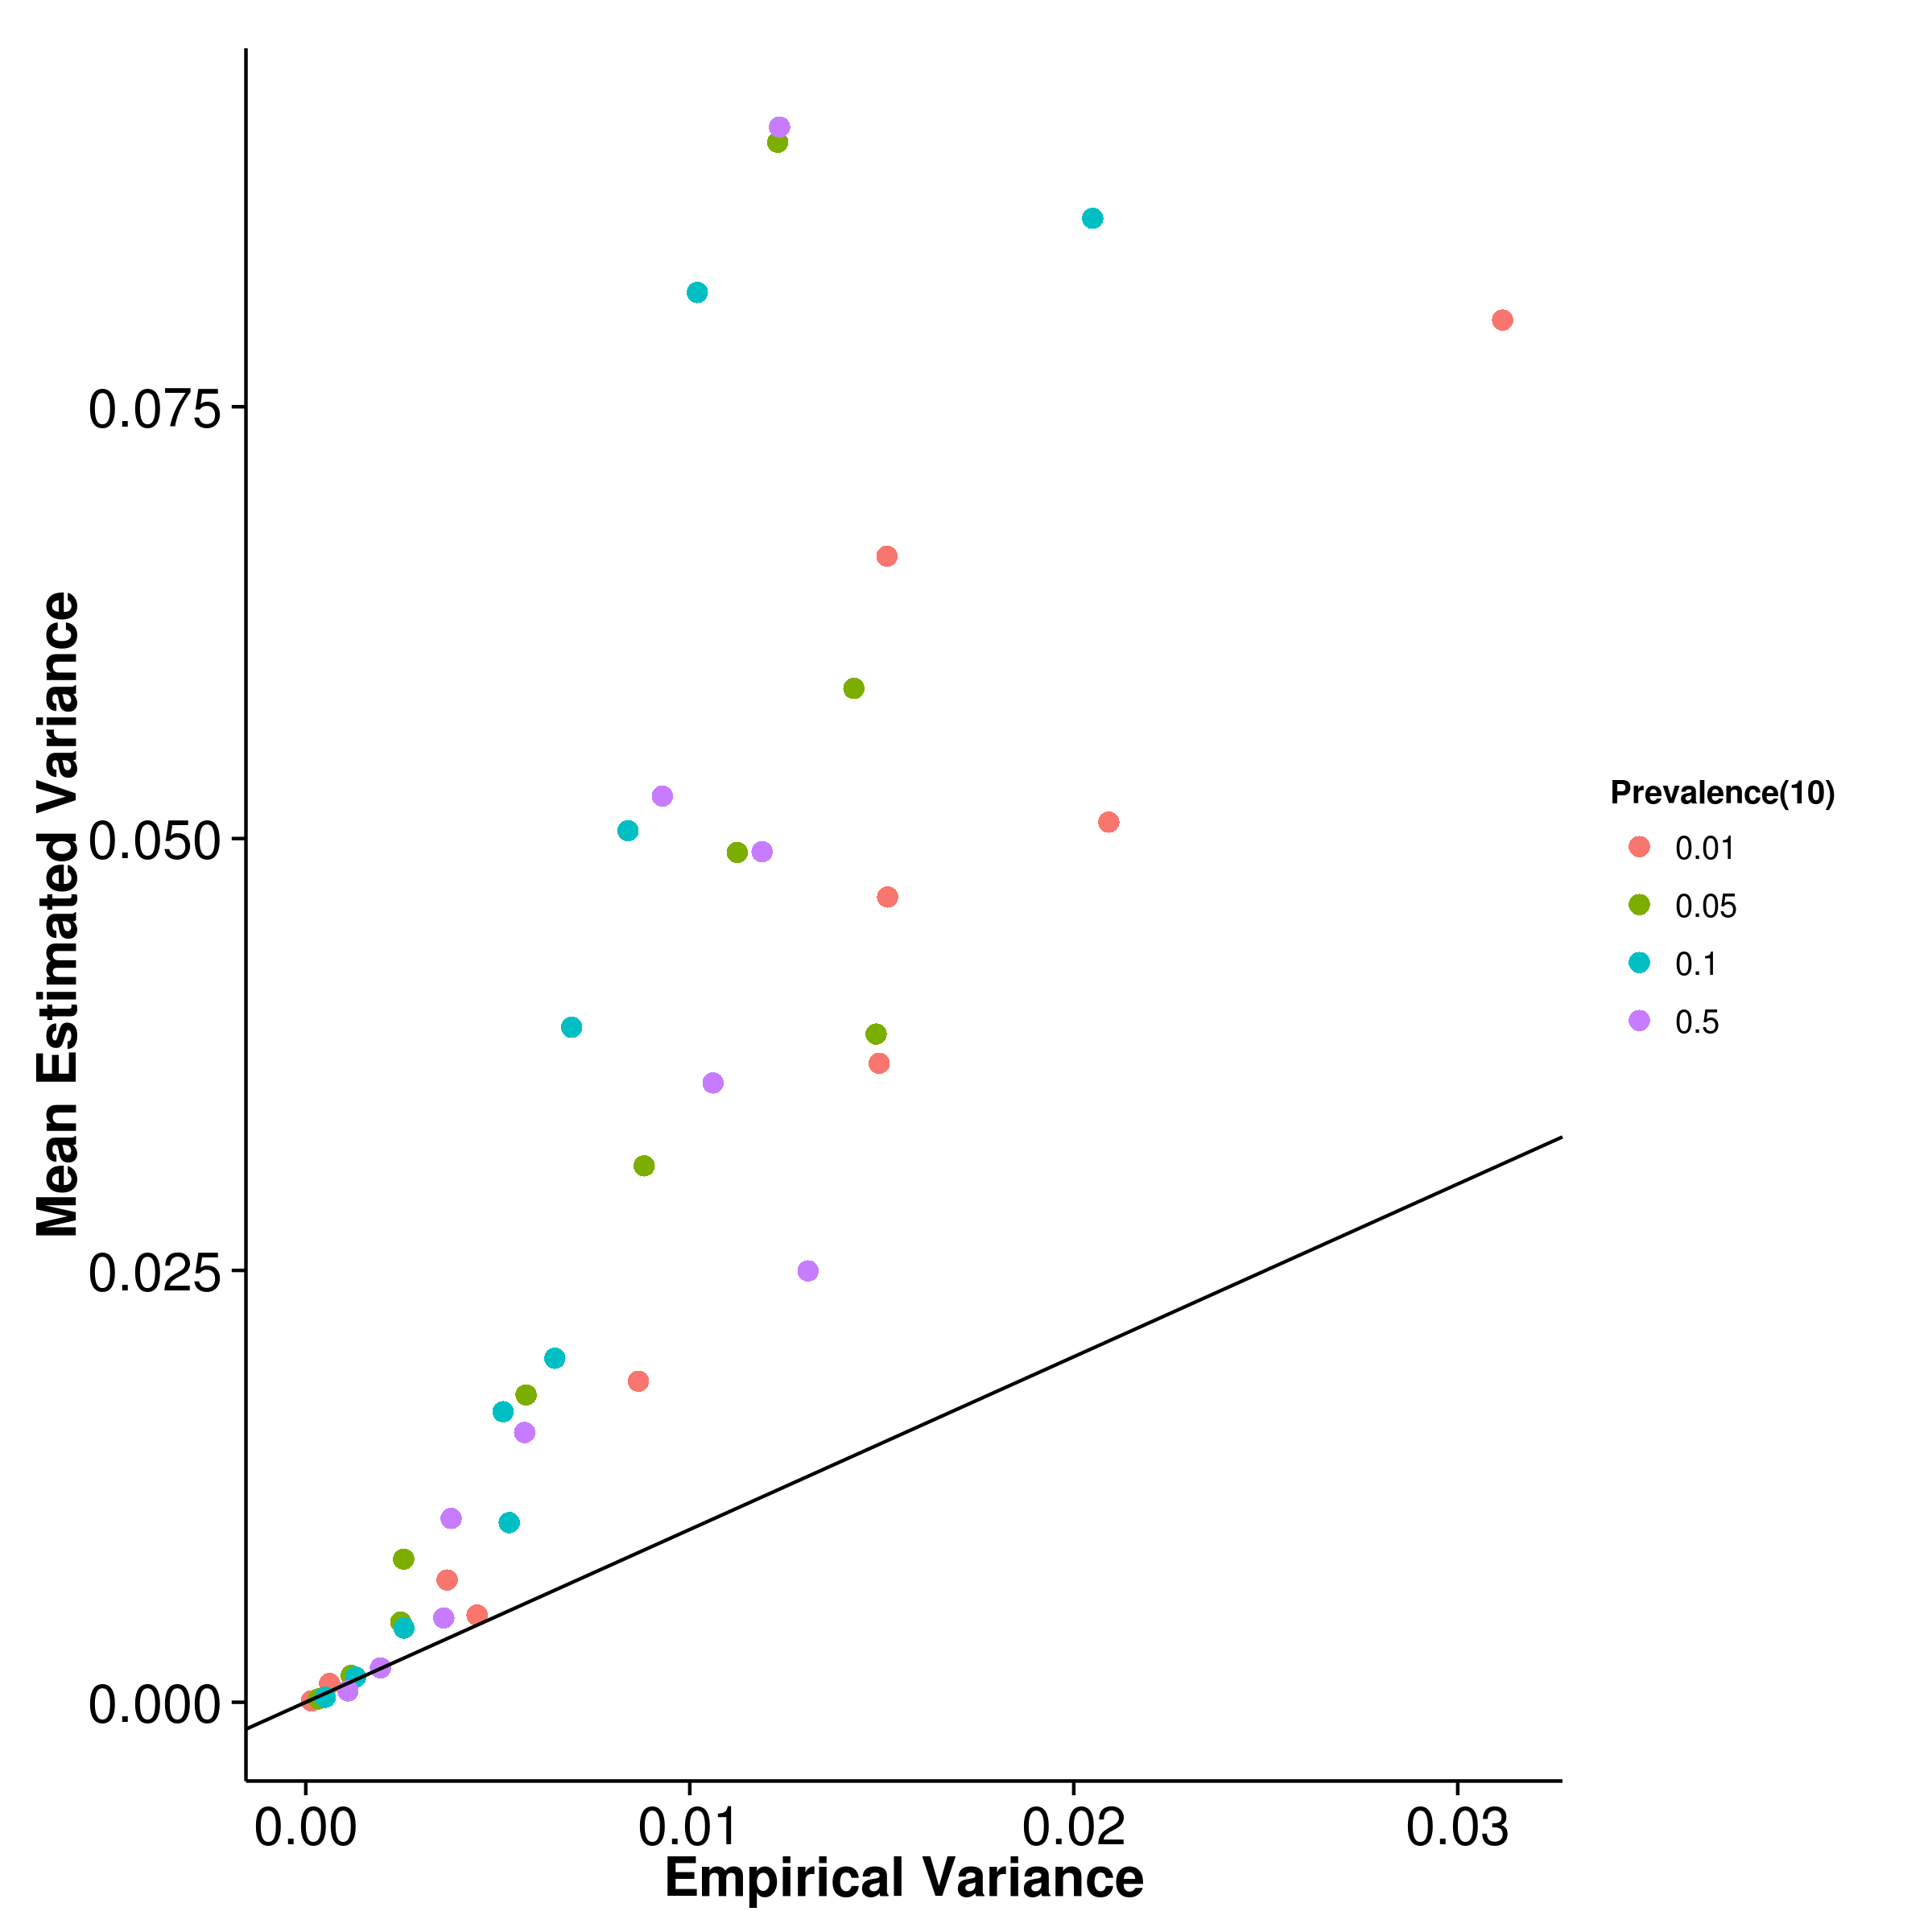
\includegraphics{figure/he_summary/cc_10c/ldsc_CC_Rand_sdCom.png}}
				\label{fig:ldscCC10RandVarCom}
			}
			\subfloat[LDSC with intercept estimation]{
				
				\scalebox{.4}{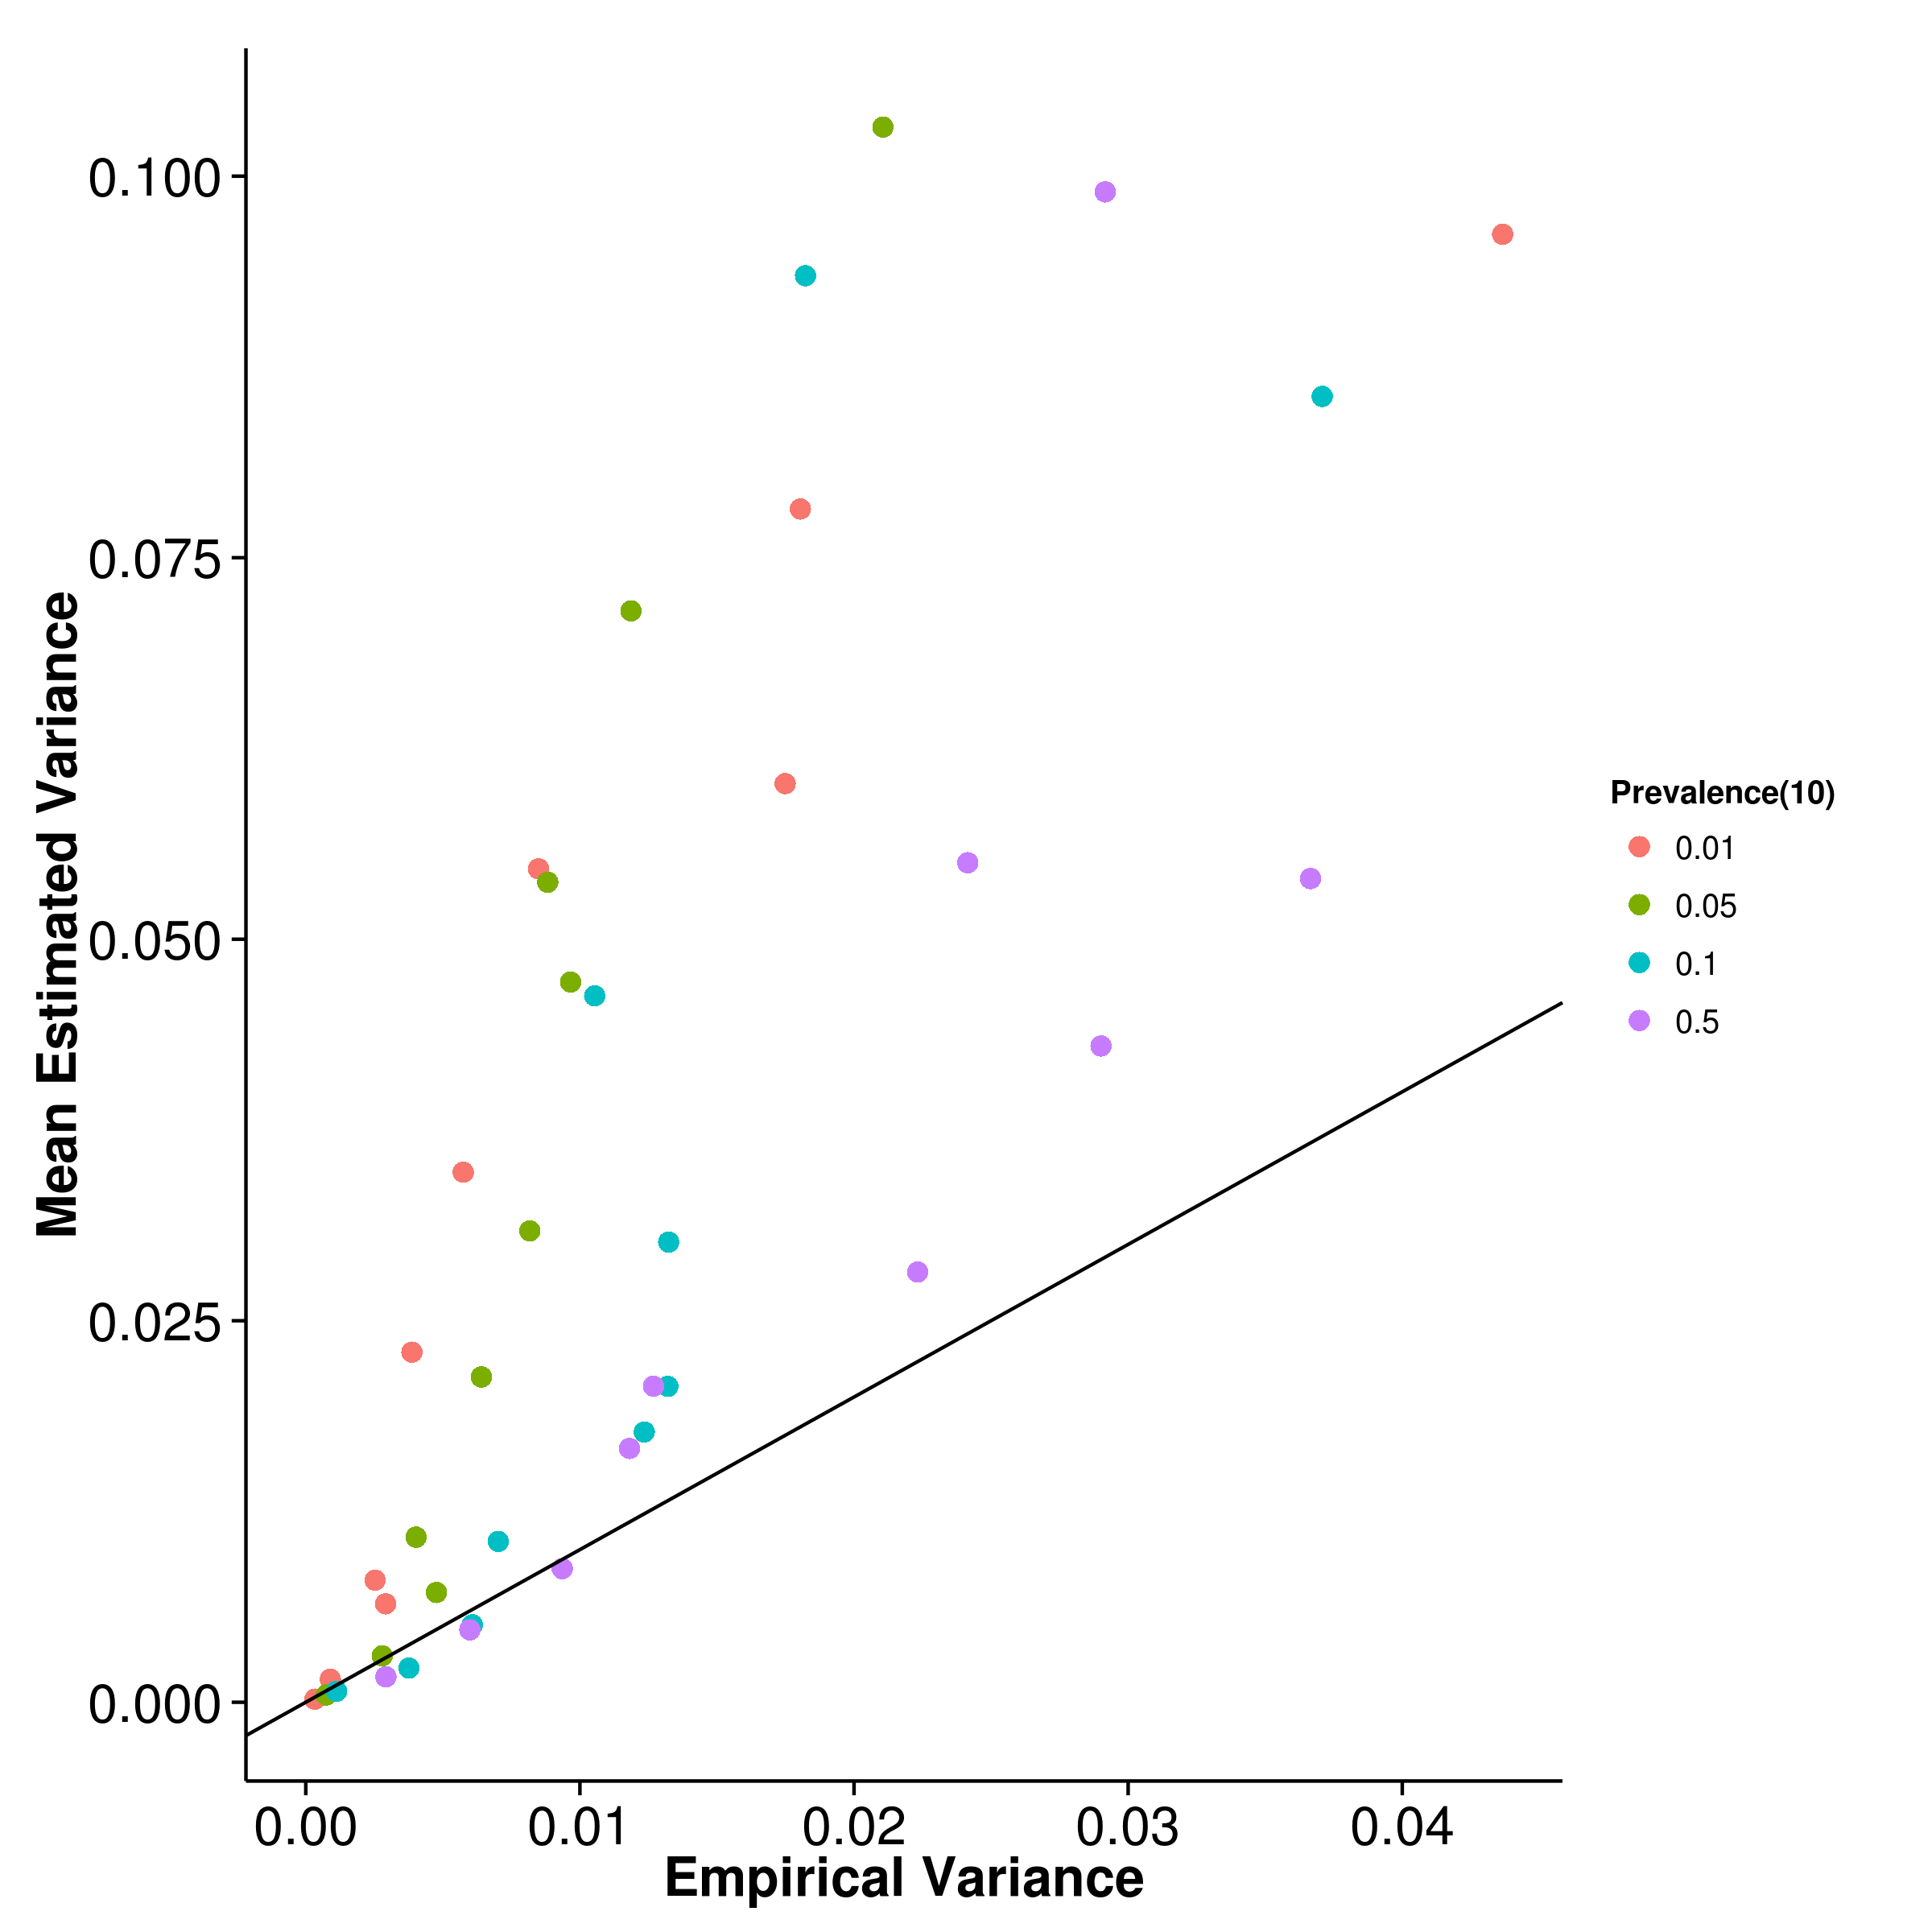
\includegraphics{figure/he_summary/cc_10c/ldscIn_CC_Rand_sdCom.png}}
				\label{fig:ldscInCC10RandVarCom}
			}
			\caption[Estimation of Variance in Case Control Simulation (10 Causal)]
			{Estimated variance of results from case control simulation with random effect size simulation when compared to empirical variance when 10 causal \glspl{SNP} was simulated.
				A general underestimation was observed for \gls{shrek} and \gls{gcta} whereas a larger upward bias was observed for \gls{ldsc}.} 
			\label{fig:CC10RandVarCom}
		\end{figure}